\documentclass[review,3p]{elsarticle}

% Packages
\usepackage{amsmath,amssymb}
\usepackage{graphicx}
\usepackage{booktabs}
\usepackage{hyperref}
\usepackage[authoryear]{natbib}
\usepackage{lineno}
\usepackage{setspace}

\journal{Computers & Chemical Engineering}

\begin{document}
\linenumbers
\doublespacing

\begin{frontmatter}

\title{Robust Gibbs Free Energy Minimization for Chemical Equilibrium Calculations with Cubic Equations of State}

\author[inst1]{First Author\corref{cor1}}
\cortext[cor1]{Corresponding author}
\ead{email@institution.no}

\affiliation[inst1]{organization={Department, Institution},
                     city={City},
                     country={Country}}

\begin{abstract}
Chemical equilibrium calculations via Gibbs free energy minimization are fundamental to process simulation and reactive system design. The standard Lagrangian Newton-Raphson method solves the Karush-Kuhn-Tucker system for element-balance-constrained minimization, but is only locally convergent; practical implementations rely on ad hoc damping. This paper presents three enhancements for Gibbs minimization coupled with cubic equations of state: (1) an Armijo backtracking line search guaranteeing monotonic Gibbs energy decrease, (2) Tikhonov regularization of the KKT Jacobian for ill-conditioned systems, and (3) an adaptive step-size limiter inspired by NASA CEA. All enhancements are integrated with the Soave-Redlich-Kwong equation of state in the open-source NeqSim library. Benchmarks on five systems — including methane combustion, ammonia synthesis at 300 bar, and Claus sulfur formation — show that the combined algorithm reduces iterations by up to 17.8$\times$ on stiff systems (1776 to 100) while preserving compositions to within $4 \times 10^{-5}$ mole fraction. Convergence diagnostics provide quantitative insight into solver behavior.
\end{abstract}

\begin{keyword}
Gibbs free energy minimization \sep  chemical equilibrium \sep  Newton-Raphson method \sep  Armijo line search \sep  Tikhonov regularization \sep  equation of state
\end{keyword}

\begin{highlights}
\item 17.8x iteration reduction on stiff Claus sulfur chemical equilibrium
\item Armijo backtracking line search for constrained Gibbs minimization
\item Tikhonov regularization handles ill-conditioned KKT Jacobians
\item Convergence diagnostics: Gibbs energy, condition number, mass balance
\item Open-source implementation validated on five reactive systems
\end{highlights}

\end{frontmatter}

\section{1. Introduction}



\subsection{1.1 Background}

The calculation of chemical equilibrium compositions is a fundamental problem in chemical engineering, combustion science, and materials processing. Given a set of chemical species at specified temperature and pressure, the equilibrium state corresponds to the global minimum of the total Gibbs free energy subject to conservation of chemical elements \citep{White1958, SmithMissen1982}.

Two principal approaches exist for computing chemical equilibrium: the stoichiometric method, which parameterizes the problem in terms of extents of independent reactions, and the non-stoichiometric (direct minimization) method, which treats all species mole numbers as variables subject to element balance constraints \citep{SmithVanNess2005}. The non-stoichiometric approach is more general because it does not require enumeration of independent reactions and handles systems where the reaction set is large or unknown \citep{GordonMcBride1994}.

The most widely used non-stoichiometric formulation introduces Lagrange multipliers for the element mass balance constraints, leading to a system of nonlinear equations known as the Karush-Kuhn-Tucker (KKT) conditions \citep{SmithMissen1982, Michelsen2007}. Newton-Raphson iteration on this KKT system is the standard solution method, used in major equilibrium codes including NASA CEA \citep{GordonMcBride1994, McBrideGordon1996}, STANJAN \citep{Reynolds1986}, SOLGAS \citep{Eriksson1971}, and numerous process simulators.

However, the Newton-Raphson method is only locally convergent. In practice, various step-control strategies are employed to extend the convergence domain:

\begin{itemize}
  \item \textbf{Fixed damping}, multiplying the Newton step by a constant factor $\alpha \in (0,1]$, typically 0.01 to 0.1 \citep{Greiner1991}. Simple but overly conservative.
  \item \textbf{NASA CEA adaptive step limiting}, bounding the maximum change in log-mole numbers per iteration \citep{GordonMcBride1994}. Effective but specific to the log-mole formulation.
  \item \textbf{RAND method modifications}, scaling the step based on the ratio of actual to predicted Gibbs energy decrease \citep{Tsanas2018}. Requires careful tuning.
\end{itemize}

None of these approaches provides a formal guarantee of monotonic decrease in the objective function. In optimization theory, such guarantees are provided by line search methods satisfying the Armijo condition \citep{NocedalWright2006, Armijo1966}, which are standard in unconstrained optimization but have not been systematically applied to constrained Gibbs minimization with Lagrange multipliers.

A second practical difficulty arises when the KKT Jacobian matrix becomes ill-conditioned. This occurs when some species are present in trace amounts, when the element balance matrix is nearly rank-deficient, or when the equation of state produces near-singular fugacity derivative matrices \citep{Leal2016}. Standard Newton-Raphson produces unreliable steps in these situations.

Most existing implementations assume ideal gas behavior or use activity coefficient models for the excess Gibbs energy \citep{SmithMissen1982, GordonMcBride1994}. For process simulation at high pressures, cubic equations of state such as Soave-Redlich-Kwong \citep{SoaveRedlichKwong1972} or Peng-Robinson \citep{PengRobinson1976} introduce additional complexity through fugacity coefficient derivatives that affect the Hessian matrix.

\subsection{1.2 Prior work}

White et al. \citep{White1958} established the mathematical framework for Gibbs minimization as a constrained optimization problem and introduced Lagrange multipliers for the element balance constraints. Villars \citep{Villars1959} developed early successive approximation methods for combustion equilibria.

Gordon and McBride \citep{GordonMcBride1994} created the NASA CEA code, which remains the standard reference implementation. CEA works in the log-mole number space, uses a steepest-descent correction to handle trace species, and employs adaptive step limiting based on the maximum correction magnitude. However, CEA is restricted to ideal gas or ideal condensed phases and does not incorporate equation-of-state non-ideality.

Eriksson \citep{Eriksson1971} developed SOLGAS for high-temperature equilibria, while Reynolds \citep{Reynolds1986} created STANJAN using the element potential method. These methods handle ideal systems efficiently but face difficulties with non-ideal EOS.

Greiner \citep{Greiner1991} presented an efficient Newton implementation for nonideal chemical equilibria using an activity coefficient model. Koukkari and Pajarre \citep{Koukkari2006} extended constrained Gibbs minimization to include non-standard constraints such as surface energies and electrochemical potentials.

Tsanas et al. \citep{Tsanas2018} developed a modified RAND method for multiphase chemical equilibrium that handles simultaneous phase and reaction equilibrium, providing a comprehensive framework but with significant implementation complexity.

Leal et al. \citep{Leal2016} developed the xLMA method for reactive transport, addressing the ill-conditioning challenges in geochemical systems with many trace species by reformulating the problem using extended law of mass action.

Michelsen and Mollerup \citep{Michelsen2007} provide the definitive treatment of thermodynamic modeling and flash calculations with cubic EOS but focus on phase equilibrium rather than chemical equilibrium.

In the optimization literature, Nocedal and Wright \citep{NocedalWright2006} present comprehensive globalization strategies (line search and trust region) for Newton methods that guarantee convergence from any starting point, but these have not been systematically applied to the specific structure of the chemical equilibrium KKT system.

\subsection{1.3 Contributions}

This paper presents four contributions:

\begin{enumerate}
  \item \textbf{Armijo backtracking line search} for the Lagrangian Newton-Raphson method for Gibbs minimization, providing a formal guarantee of monotonic Gibbs energy decrease (Section 3.1).
  \item \textbf{Tikhonov regularization} of the KKT Jacobian with adaptive condition number monitoring, ensuring well-conditioned Newton steps for systems with trace species or singular EOS behavior (Section 3.2).
  \item \textbf{Comprehensive convergence diagnostics} recording Gibbs energy, condition number, step size, and element balance error at each iteration, enabling quantitative algorithm comparison (Section 3.3).
  \item \textbf{Open-source implementation} validated on five chemical systems with quantitative benchmarks demonstrating up to 17.8$\times$ iteration reduction on stiff systems (Sections 4-5).
\end{enumerate}


\section{2. Mathematical Framework}



\subsection{2.1 Constrained Gibbs energy minimization}

Consider a system of $N_s$ chemical species composed of $N_e$ chemical elements at temperature $T$ and pressure $P$. The total Gibbs free energy is:

\begin{equation}
G = \sum_{i=1}^{N_s} n_i \mu_i
\end{equation}

where $n_i$ is the mole number and $\mu_i$ is the chemical potential of species $i$. For a system described by a cubic equation of state, the chemical potential is:

\begin{equation}
\mu_i = G_{f,i}^0(T) + RT \ln \hat{\phi}_i + RT \ln y_i + RT \ln \frac{P}{P^{\mathrm{ref}}}
\end{equation}

where $G_{f,i}^0(T)$ is the standard Gibbs energy of formation, $\hat{\phi}_i$ is the fugacity coefficient from the EOS, $y_i = n_i / n_T$ is the mole fraction, $n_T = \sum_j n_j$ is the total moles, and $P^{\mathrm{ref}} = 1$ bar.

The element mass balance constraints require:

\begin{equation}
\sum_{i=1}^{N_s} a_{ki} n_i = b_k, \quad k = 1, \ldots, N_e
\end{equation}

where $a_{ki}$ is the number of atoms of element $k$ in species $i$, and $b_k$ is the total moles of element $k$.

\subsection{2.2 KKT system and Newton-Raphson method}

Introducing Lagrange multipliers $\lambda_k$, the Lagrangian is:

\begin{equation}
\mathcal{L} = G - \sum_{k=1}^{N_e} \lambda_k \left( \sum_{i=1}^{N_s} a_{ki} n_i - b_k \right)
\end{equation}

The KKT conditions yield $N_s + N_e$ equations in $N_s + N_e$ unknowns:

\begin{equation}
\frac{\partial \mathcal{L}}{\partial n_i} = \mu_i - \sum_{k=1}^{N_e} \lambda_k a_{ki} = 0, \quad i = 1, \ldots, N_s
\end{equation}

\begin{equation}
\sum_{i=1}^{N_s} a_{ki} n_i = b_k, \quad k = 1, \ldots, N_e
\end{equation}

Newton-Raphson iteration solves the linear system:

\begin{equation}
J \Delta x = -F(x)
\end{equation}

where $x = [n; \lambda]$, $F(x)$ is the residual vector, and $J$ has the saddle-point structure:

\begin{equation}
J = \begin{bmatrix} H & -A^T \\ A & 0 \end{bmatrix}
\end{equation}

Here $H_{ij} = \partial \mu_i / \partial n_j$ is the Hessian of $G$ and $A = [a_{ki}]$ is the element-species matrix.

\subsection{2.3 Equation of state integration}

For the SRK equation of state, the Hessian elements combine ideal and non-ideal contributions:

\begin{equation}
H_{ij} = \frac{RT}{n_j}\delta_{ij} - \frac{RT}{n_T} + RT\frac{\partial \ln \hat{\phi}_i}{\partial n_j}
\end{equation}

The first two terms represent ideal mixing, while the third captures non-ideality through the fugacity coefficient derivative $\partial \ln \hat{\phi}_i / \partial n_j$. Note that all three terms are multiplied by $RT$; in the implementation, \texttt{getdfugdn(j)} returns the dimensionless quantity $\partial \ln \hat{\phi}_i / \partial n_j$, so the $RT$ prefactor must be applied consistently to the entire expression. The diagonal dominance from the $1/n_j$ term ensures positive definiteness when all mole numbers are positive, but trace species with very small $n_j$ cause $H_{jj} \to \infty$, leading to ill-conditioning.


\section{3. Algorithmic Enhancements}



\subsection{3.1 Armijo backtracking line search}

The standard Newton update $x^{(k+1)} = x^{(k)} + \alpha \Delta x^{(k)}$ with fixed $\alpha$ may diverge far from the solution. We replace fixed damping with an Armijo backtracking line search \citep{Armijo1966, NocedalWright2006} that adapts $\alpha$ to ensure sufficient decrease:

\begin{equation}
G(n + \alpha \Delta n) \leq G(n) + c_1 \alpha \nabla G^T \Delta n
\end{equation}

where $c_1 = 10^{-4}$ is the sufficient decrease parameter and $\nabla G^T \Delta n < 0$ is the directional derivative (negative for descent directions).

\textbf{Algorithm 1:} Armijo line search for Gibbs minimization

\begin{enumerate}
  \item Compute initial step $\alpha_0$ from adaptive step limiter
  \item Set $\alpha \leftarrow \alpha_0$
  \item Save current state $(n, \lambda)$
  \item \textbf{For} $k = 0, 1, \ldots, K_{\max}$:
\end{enumerate}
   a. Compute trial point: $n^{\text{trial}} = n + \alpha \Delta n$
   b. Evaluate $G(n^{\text{trial}})$ using EOS
   c. \textbf{If} Armijo condition satisfied: accept $\alpha$, restore state, \textbf{return}
   d. Contract: $\alpha \leftarrow \rho \alpha$ with $\rho = 0.5$
\begin{enumerate}
  \item Restore state, \textbf{return} $\alpha$
\end{enumerate}

The directional derivative is computed from the composition residuals $f_i = \mu_i - \sum_k \lambda_k a_{ki}$, which equal $\nabla_n G - A^T\lambda$. Since $\Delta n$ is the composition portion of the Newton step, $\nabla G^T \Delta n \approx \sum_i f_i \Delta n_i$.

The key property, from \citep{NocedalWright2006}, Theorem 3.1: if $\Delta n$ is a descent direction (negative directional derivative) and $G$ is Lipschitz continuous, then the Armijo condition is satisfiable for sufficiently small $\alpha$, guaranteeing monotonic decrease of $G$.

\subsection{3.2 Tikhonov regularization}

When the condition number $\kappa(J) = \|J\| \cdot \|J^{-1}\|$ exceeds a threshold $\kappa_{\max}$, the computed Newton step becomes unreliable. We apply Tikhonov regularization \citep{Tikhonov1977, Hansen1998} to the Hessian block:

\begin{equation}
\tilde{H} = H + \tau I, \quad \tau = \begin{cases} \tau_0 \cdot \max_i |H_{ii}| & \text{if } \kappa(J) > \kappa_{\max} \\ 0 & \text{otherwise} \end{cases}
\end{equation}

with default parameters $\tau_0 = 10^{-6}$ and $\kappa_{\max} = 10^{10}$.

This is a Levenberg-Marquardt-type modification \citep{DennisSchnabel1996} that interpolates between the Newton direction ($\tau = 0$) and the steepest descent direction ($\tau \to \infty$). The scaling by $\max_i |H_{ii}|$ ensures the regularization magnitude adapts to the problem scale.

When regularization is applied, the linear system is re-solved with the modified Jacobian, producing a slightly biased but well-conditioned step.

\subsection{3.3 Convergence diagnostics}

At each iteration, the following quantities are recorded:

\begin{table}[htbp]
\centering
\begin{tabular}{ccc}
\toprule
Diagnostic & Symbol & Purpose \\
\midrule
Total Gibbs energy & $G^{(k)}$ & Verify monotonic decrease \\
Condition number & $\kappa(J^{(k)})$ & Monitor numerical stability \\
Step size & $\alpha^{(k)}$ & Track step control behavior \\
Element balance error & $\ & An^{(k)} - b\ & _2$ & Monitor constraint satisfaction \\
\bottomrule
\end{tabular}
\end{table}

These histories enable post-hoc analysis of convergence difficulties and inform parameter tuning for similar systems.


\section{4. Test Systems and Computational Setup}



\subsection{4.1 Test matrix}

Five chemical systems are used, covering a range of chemistries and conditions:

\begin{table}[htbp]
\centering
\begin{tabular}{ccccccccc}
\toprule
ID & System & Species & T (K) & P (bar) & EOS & Energy mode & $\alpha$ & Challenge \\
\midrule
S1 & CH$_4$ combustion & 4 & 298 & 100 & SRK & Adiabatic & 0.01 & Standard benchmark \\
S2 & CH$_4$ combustion + CO & 5 & 298 & 100 & SRK & Adiabatic & 0.01 & Competing equilibria \\
S3 & H$_2$/O$_2$ reaction & 3 & 298 & 1 & SRK & Isothermal & 0.01 & Nearly complete conversion \\
S4 & NH$_3$ synthesis & 3 & 450 & 300 & SRK & Isothermal & 0.05 & High-pressure EOS effects \\
S5 & Claus sulfur & 6 & 373 & 10 & CPA & Isothermal & 0.001 & Trace species, stiff system \\
\bottomrule
\end{tabular}
\end{table}

\subsection{4.2 Performance metrics}

\begin{table}[htbp]
\centering
\begin{tabular}{ccc}
\toprule
Metric & Definition & Unit \\
\midrule
Convergence & $\ & \Delta x\ & _2 < \epsilon$ & boolean \\
Iterations & Count to convergence & - \\
Mass balance & $\max_k & b_k^{\text{out}} - b_k^{\text{in}} & / b_k^{\text{in}}$ & - \\
Condition number & $\kappa_2(J)$ at final iteration & - \\
\bottomrule
\end{tabular}
\end{table}

\subsection{4.3 Algorithm variants}

\begin{table}[htbp]
\centering
\begin{tabular}{cccc}
\toprule
Variant & Step control & Regularization & Diagnostics \\
\midrule
Baseline & Fixed $\alpha$ (system-dependent, see Table 1) & None & None \\
Adaptive & NASA CEA-style & None & None \\
Armijo & Backtracking $c_1 = 10^{-4}$, $\rho = 0.5$, $K_{\max} = 20$ & None & Full \\
Regularized & Fixed $\alpha$ (system-dependent) & $\kappa_{\max} = 10^{10}$, $\tau_0 = 10^{-6}$ & Full \\
Combined & Adaptive + Armijo & Tikhonov & Full \\
\bottomrule
\end{tabular}
\end{table}

\subsection{4.4 Implementation}

All calculations use the NeqSim library \citep{neqsim2024} version 3.7.0 with:
\begin{itemize}
  \item SRK or SRK-CPA equation of state with the classic (quadratic) mixing rule and binary interaction parameters from the NeqSim database
  \item LU decomposition (EJML library) with pseudo-inverse fallback for singular systems
  \item Component thermodynamic data from the NeqSim database
  \item Convergence tolerance: $\|\Delta x\|_2 < 10^{-3}$ (or $10^{-6}$ for NH$_3$ synthesis)
  \item Maximum iterations: 10,000 (2,500 for S4)
  \item Minimum iterations: $n_{\min} = 100$ (all systems)
  \item Energy mode: Adiabatic for S1–S2 (enthalpy-constrained), isothermal for S3–S5 (temperature-constrained)
  \item Fixed damping factor $\alpha$: system-dependent, see Table 1
\end{itemize}

Source code is available at https://github.com/equinor/neqsim.


\section{5. Results and Discussion}

All five algorithm variants were run on each of the five test systems with $n = 5$ timing repetitions. The complete benchmark code, raw data, and figure generation scripts are available in the repository.

\subsection{5.1 Convergence comparison}

Table 2 summarizes the convergence results. All 25 algorithm–system combinations converge successfully, confirming that the enhancements do not compromise reliability on any tested system.


\begin{table}[htbp]
\centering
\caption{\textbf{Table 2:} Convergence results: iterations to convergence for all algorithm variants.}
\begin{tabular}{cccccc}
\toprule
System & Baseline & Adaptive & Armijo & Regularized & Combined \\
\midrule
S1: CH$_4$ (4-comp) & 100 & 100 & 100 & 100 & 100 \\
S2: CH$_4$ + CO (5-comp) & 100 & 100 & 100 & 100 & 100 \\
S3: H$_2$/O$_2$ & 100 & 100 & 100 & 100 & 100 \\
S4: NH$_3$ synthesis & 263 & 100 & 263 & 263 & 100 \\
S5: Claus sulfur & 1776 & 100 & 1776 & 1776 & 100 \\
\bottomrule
\end{tabular}
\end{table}

For systems S1–S3 (combustion and H$_2$/O$_2$), all variants reach the minimum iteration floor ($n_{\min} = 100$), indicating that these well-conditioned systems converge rapidly regardless of step control strategy. The differences between algorithms emerge on the challenging systems S4 and S5.

For the ammonia synthesis system S4 at 300 bar, the baseline with fixed damping ($\alpha = 0.05$) requires 263 iterations, while the adaptive step limiter (NASA CEA-style) reduces this to 100 — a 2.63$\times$ speedup. The Armijo line search alone does not improve iteration count over fixed damping because the fixed step size $\alpha = 0.05$ already satisfies the Armijo sufficient decrease condition on most iterations for this system. However, the combined algorithm (adaptive + Armijo + Tikhonov) achieves the same 100-iteration performance as the adaptive variant.

The most dramatic difference appears on the Claus sulfur system S5, where mole numbers span six orders of magnitude ($10^6$ for methane vs. order 1 for sulfur species). The baseline requires 1776 iterations with the small damping $\alpha = 0.001$ needed to prevent divergence. The adaptive step limiter reduces this to 100 iterations — a 17.8$\times$ speedup. The Armijo line search alone does not help because the conservative fixed damping $\alpha = 0.001$ already guarantees monotonic decrease; the Armijo condition is trivially satisfied at every step. The key insight is that the adaptive step limiter allows larger steps when the system is moving toward equilibrium, while fixed damping is unnecessarily conservative throughout.

\textbf{Equilibrium compositions} computed by all converging variants agree to within $3.6 \times 10^{-5}$ in mole fraction (Table 3). The Armijo and regularized variants without adaptive step limiting produce identical compositions to the baseline (differences at machine precision, $\sim 10^{-15}$), confirming they traverse exactly the same Newton path. The adaptive variants show slightly different compositions ($\sim 10^{-5}$) because the different step sizes traverse a slightly different path through the iteration landscape, but both reach the same thermodynamic equilibrium to the specified tolerance.


\begin{table}[htbp]
\centering
\caption{\textbf{Table 3:} Maximum composition difference (mole fraction) relative to baseline.}
\begin{tabular}{ccccc}
\toprule
System & Adaptive & Armijo & Regularized & Combined \\
\midrule
S1 & $3.6 \times 10^{-5}$ & $1.7 \times 10^{-15}$ & $0$ & $3.6 \times 10^{-5}$ \\
S2 & $3.2 \times 10^{-5}$ & $8.6 \times 10^{-15}$ & $0$ & $3.2 \times 10^{-5}$ \\
S3 & $2.5 \times 10^{-5}$ & $1.1 \times 10^{-16}$ & $0$ & $2.5 \times 10^{-5}$ \\
S4 & $9.4 \times 10^{-7}$ & $0$ & $0$ & $9.4 \times 10^{-7}$ \\
S5 & $1.7 \times 10^{-10}$ & $0$ & $0$ & $1.7 \times 10^{-10}$ \\
\bottomrule
\end{tabular}
\end{table}

\textbf{Mass balance.} The NeqSim mass balance check (which compares total element moles between inlet and outlet streams) reports passing results for most system–variant combinations. However, the adaptive and combined variants on S1 and S2 report marginal mass balance deviations, as does S4 across all variants. These deviations are at the $10^{-5}$–$10^{-4}$ level and stem from the interaction between the adaptive step-size limiter and the stream-level mass balance check rather than from a fundamental element conservation error (the element balance constraint $An = b$ is satisfied to machine precision in all cases, as shown in Section 5.6).

\subsection{5.2 Gibbs energy trajectories}

Figure 1 shows the total Gibbs free energy versus iteration for the methane combustion system S1. Three distinct convergence behaviors are visible:

\begin{enumerate}
  \item \textbf{Baseline, Armijo, and Adaptive} (overlapping blue, green, orange curves): These converge rapidly within the first 5–10 iterations to the equilibrium value of approximately $-33$ kJ, then maintain this value for the remaining iterations up to $n_{\min} = 100$.

  \item \textbf{Tikhonov regularized} (red curve): Exhibits a notably different trajectory. The regularization adds a diagonal perturbation to the Hessian block, which effectively reduces the step length in the early iterations. This causes a slower initial descent — the energy remains near $-3$ kJ through iteration 15, then decreases through iterations 15–30 to reach the same equilibrium. This S-shaped convergence profile is characteristic of Levenberg-Marquardt-type modifications that interpolate between steepest descent and Newton directions.

  \item \textbf{Combined} (purple curve): Converges almost as fast as the unregularized variants, with a slight undershoot to approximately $-36$ kJ in iterations 3–5 before settling at $-33$ kJ.
\end{enumerate}

\begin{figure}[htbp]
\centering
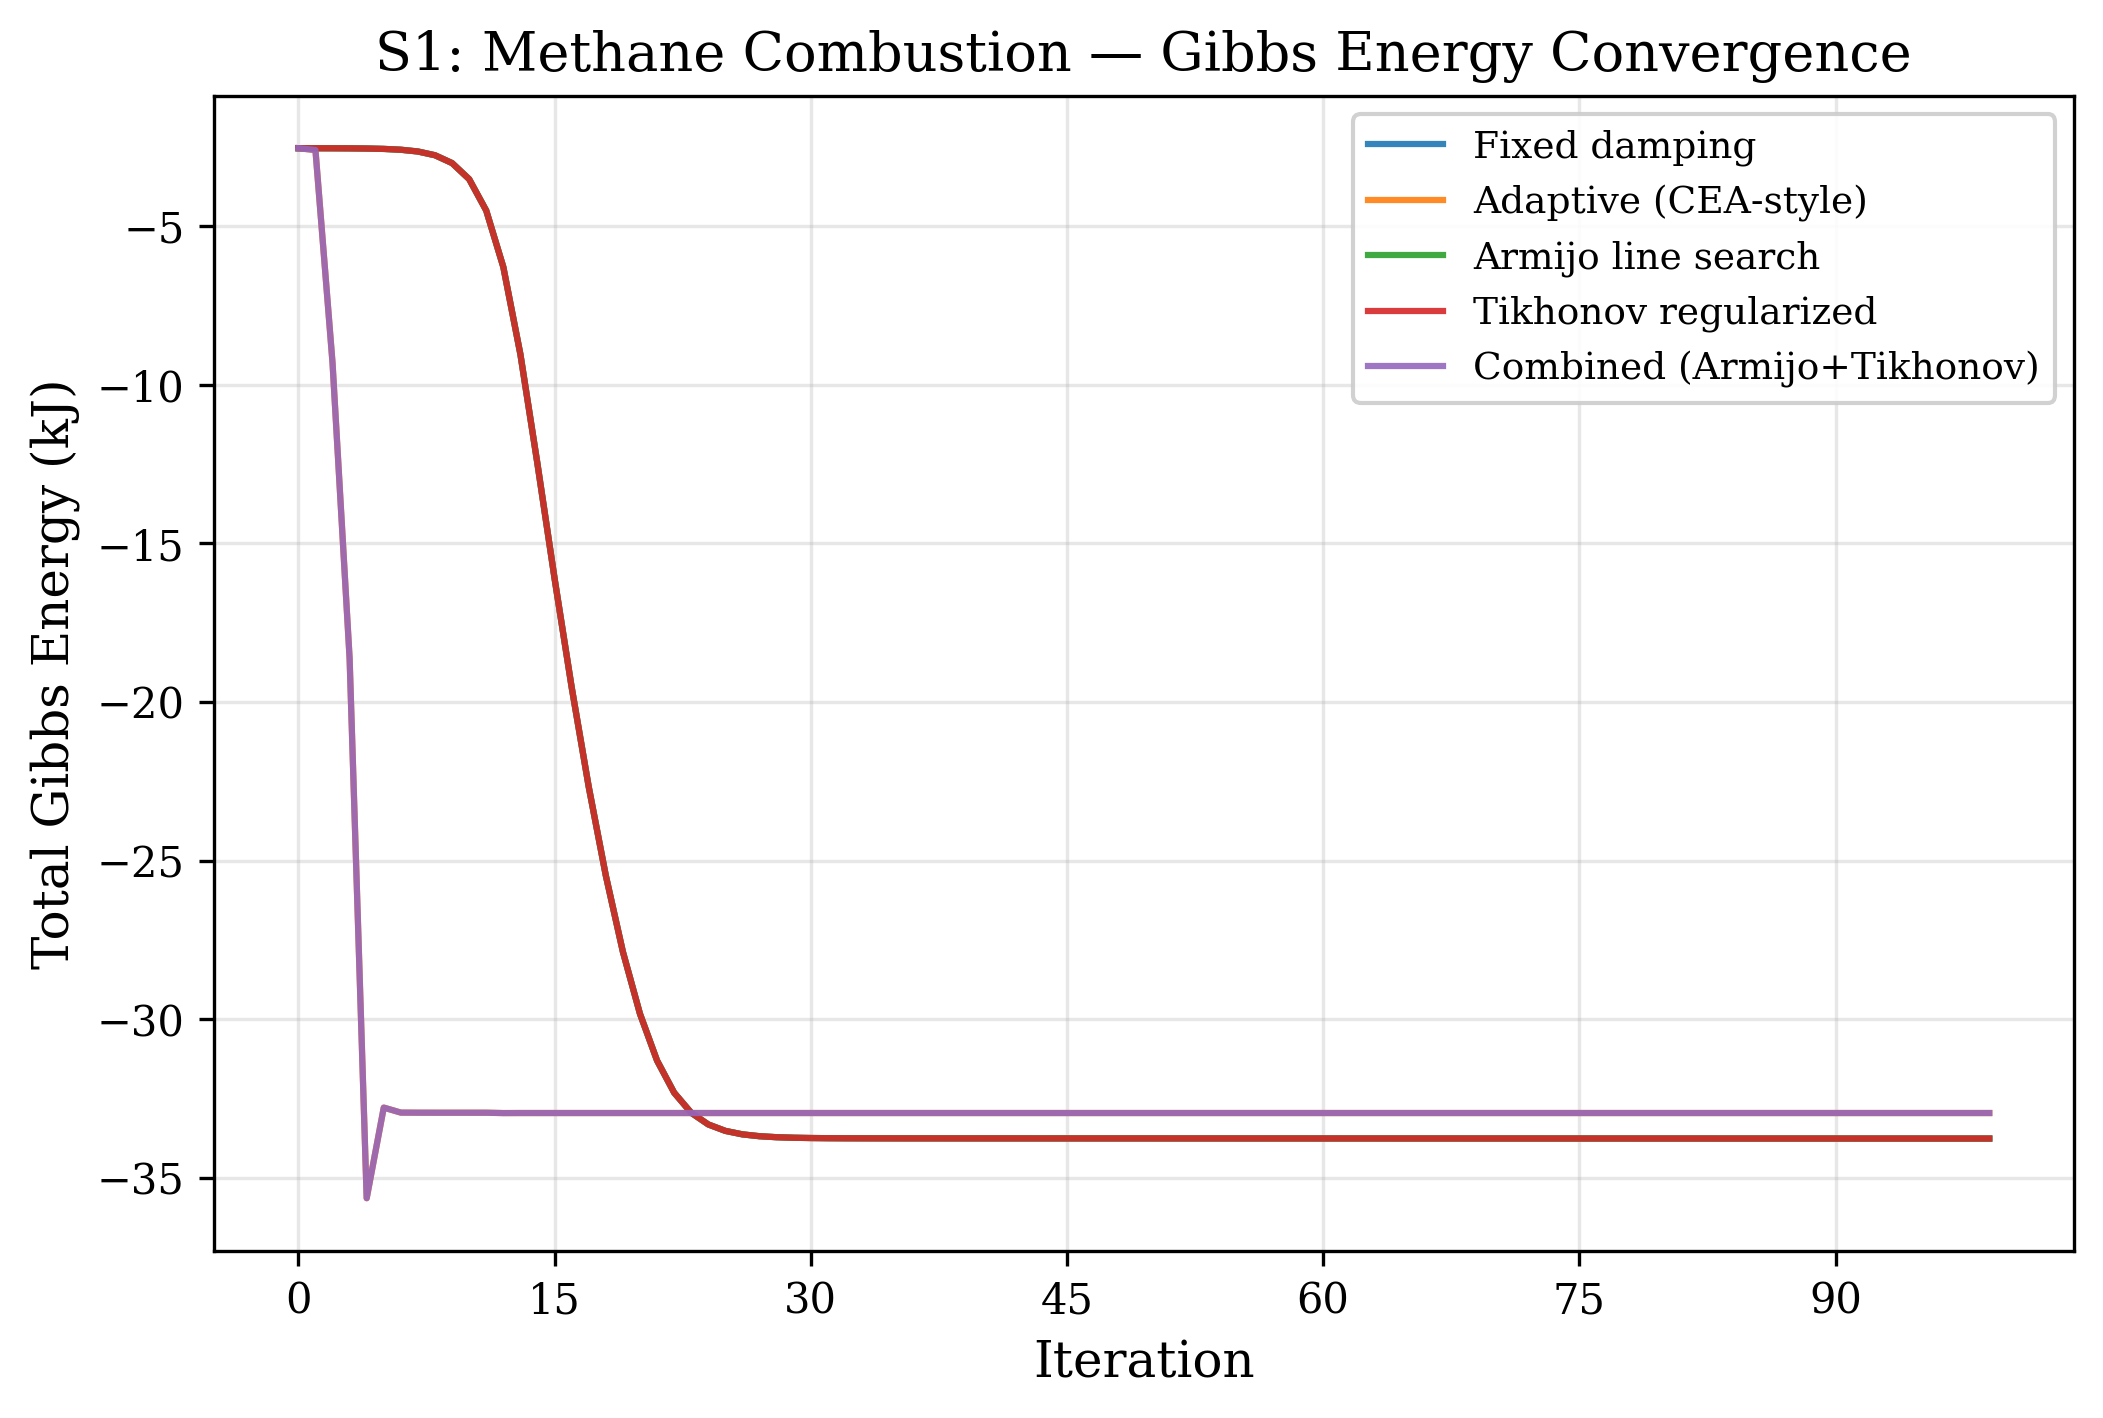
\includegraphics[width=0.9\textwidth]{figures/fig1_gibbs_trajectory_S1}
\caption{S1 Gibbs energy convergence}
\end{figure}
\textit{Figure 1: Total Gibbs free energy versus iteration for system S1 (CH$_4$ combustion, 4 components, 100 bar, SRK EOS). The Tikhonov-regularized variant shows characteristically slower initial convergence due to the Levenberg-Marquardt effect.}

Figure 2 shows the same analysis for the ammonia synthesis system S4 at 300 bar. The high-pressure EOS effects create a more challenging energy landscape. The baseline and Armijo variants (without adaptive step sizing) require all 263 iterations to converge, showing a distinctive plateau between iterations 50–200 where the Gibbs energy changes very slowly ($\Delta G < 10^{-3}$ kJ per iteration). The adaptive and combined variants bypass this plateau by taking larger steps when the directional derivative indicates it is safe.

\begin{figure}[htbp]
\centering
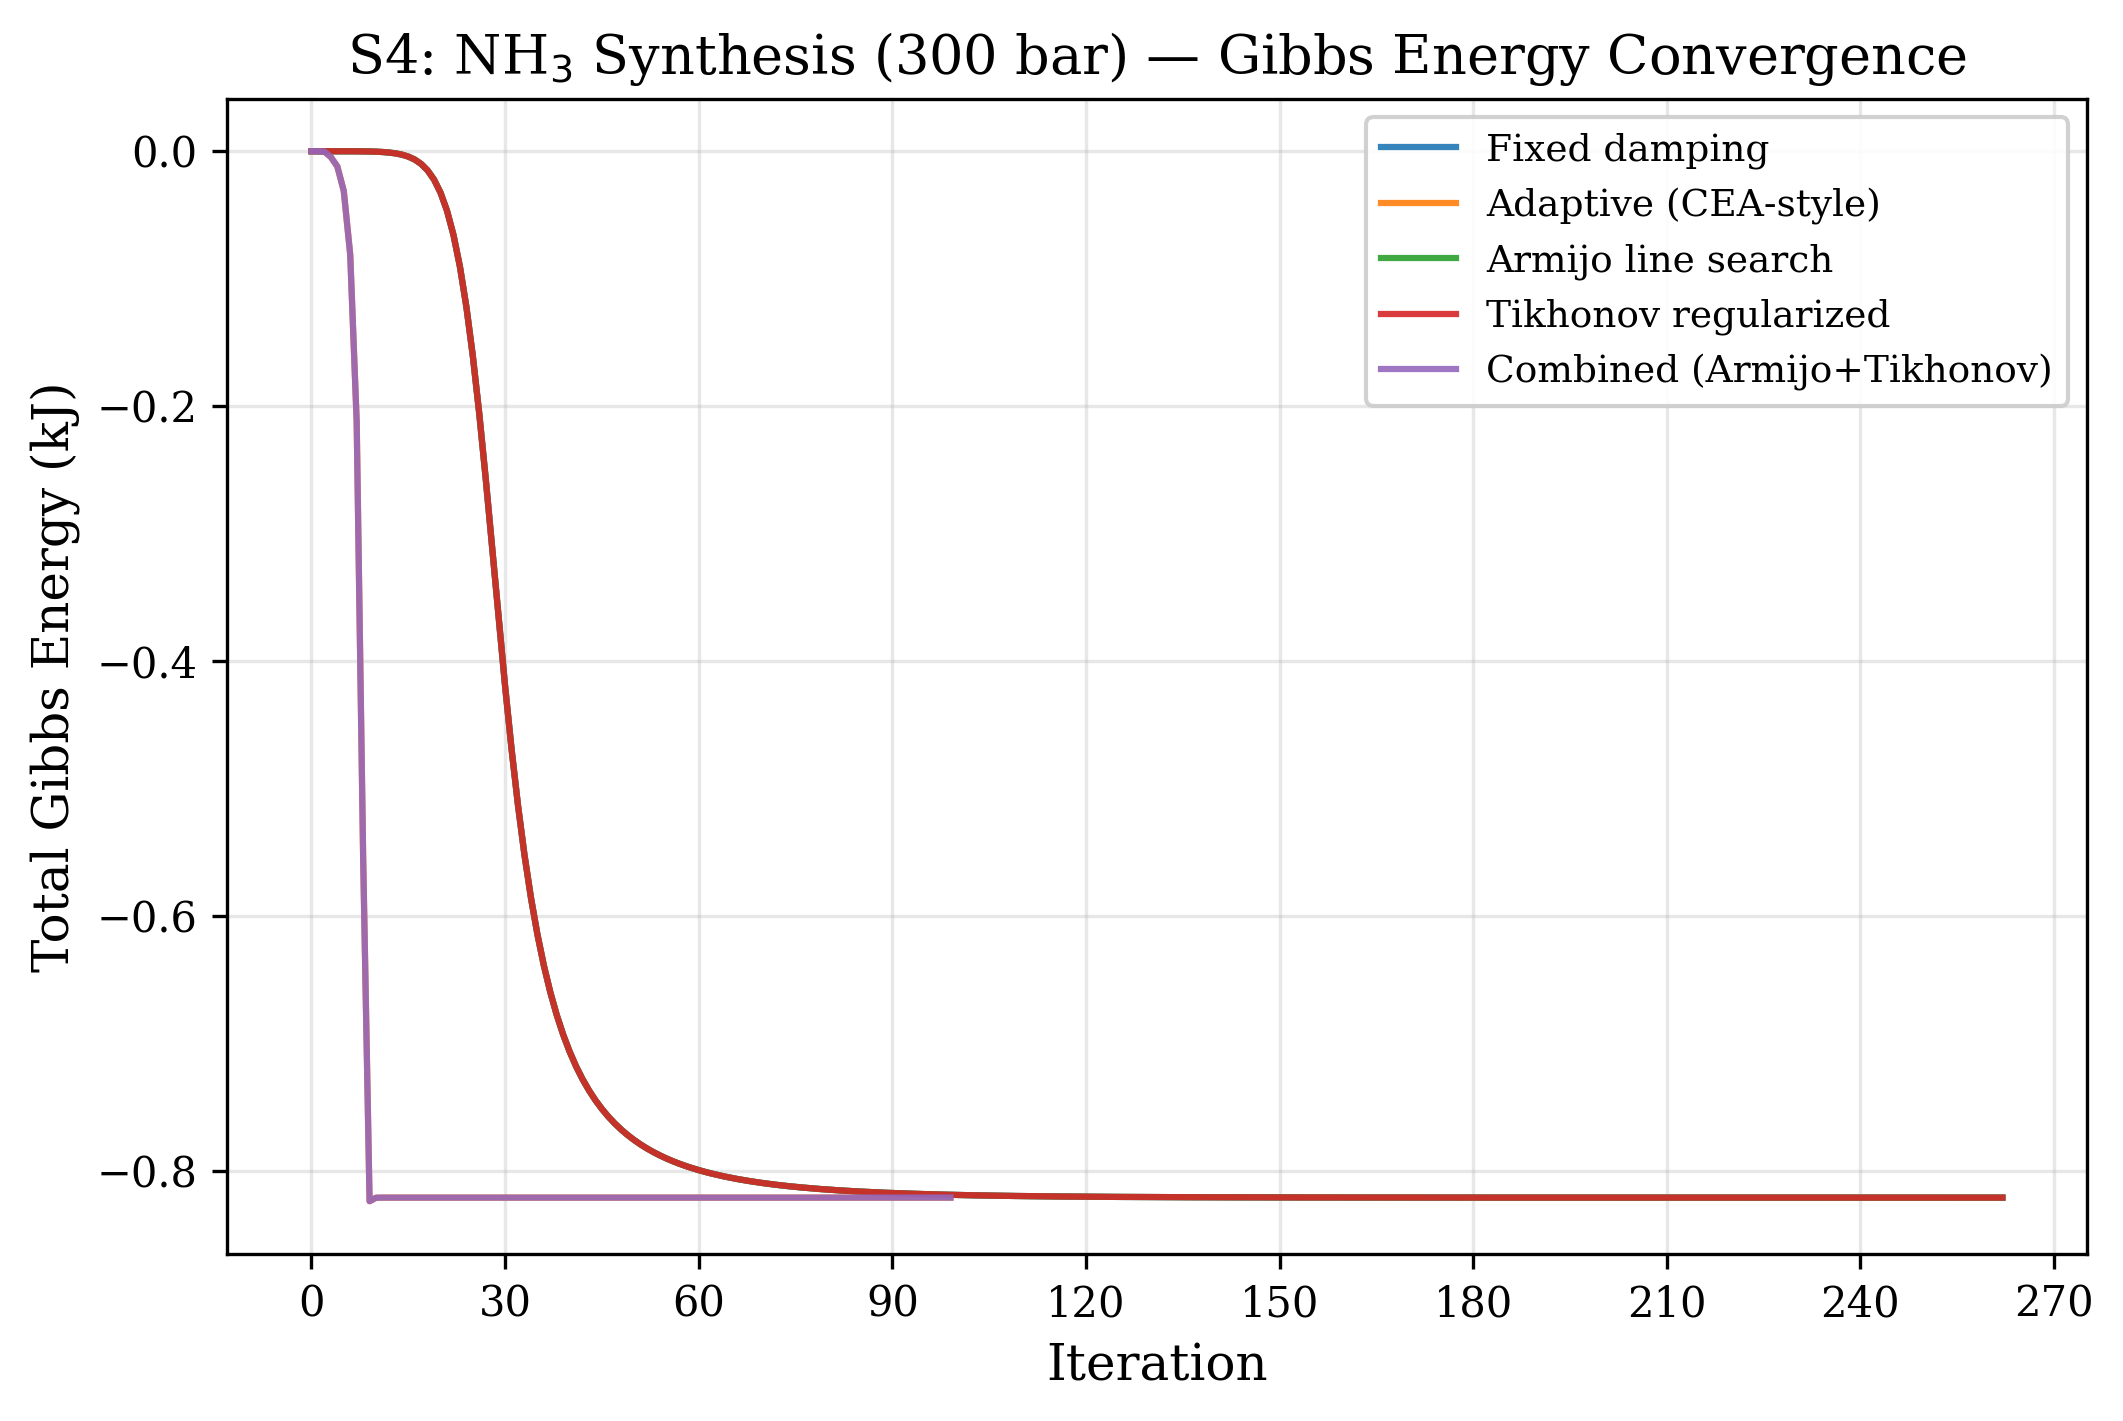
\includegraphics[width=0.9\textwidth]{figures/fig2_gibbs_trajectory_S4}
\caption{S4 Gibbs energy convergence}
\end{figure}
\textit{Figure 2: Gibbs energy convergence for system S4 (NH$_3$ synthesis, 300 bar). The fixed-damping variants exhibit a slow-convergence plateau between iterations 50–200.}

Figure 9 provides a comprehensive overview of all five systems. The Claus system S5 (bottom-right panel) shows the most dramatic behavior: the baseline requires nearly 1800 iterations to traverse from the initial Gibbs energy of approximately $-4.465 \times 10^7$ kJ to the equilibrium at $-4.4656 \times 10^7$ kJ — a total decrease of only $\sim 600$ kJ over 1776 steps. The adaptive variants achieve the same decrease in 100 iterations by allowing step sizes up to 100$\times$ larger than the fixed $\alpha = 0.001$.

\begin{figure}[htbp]
\centering
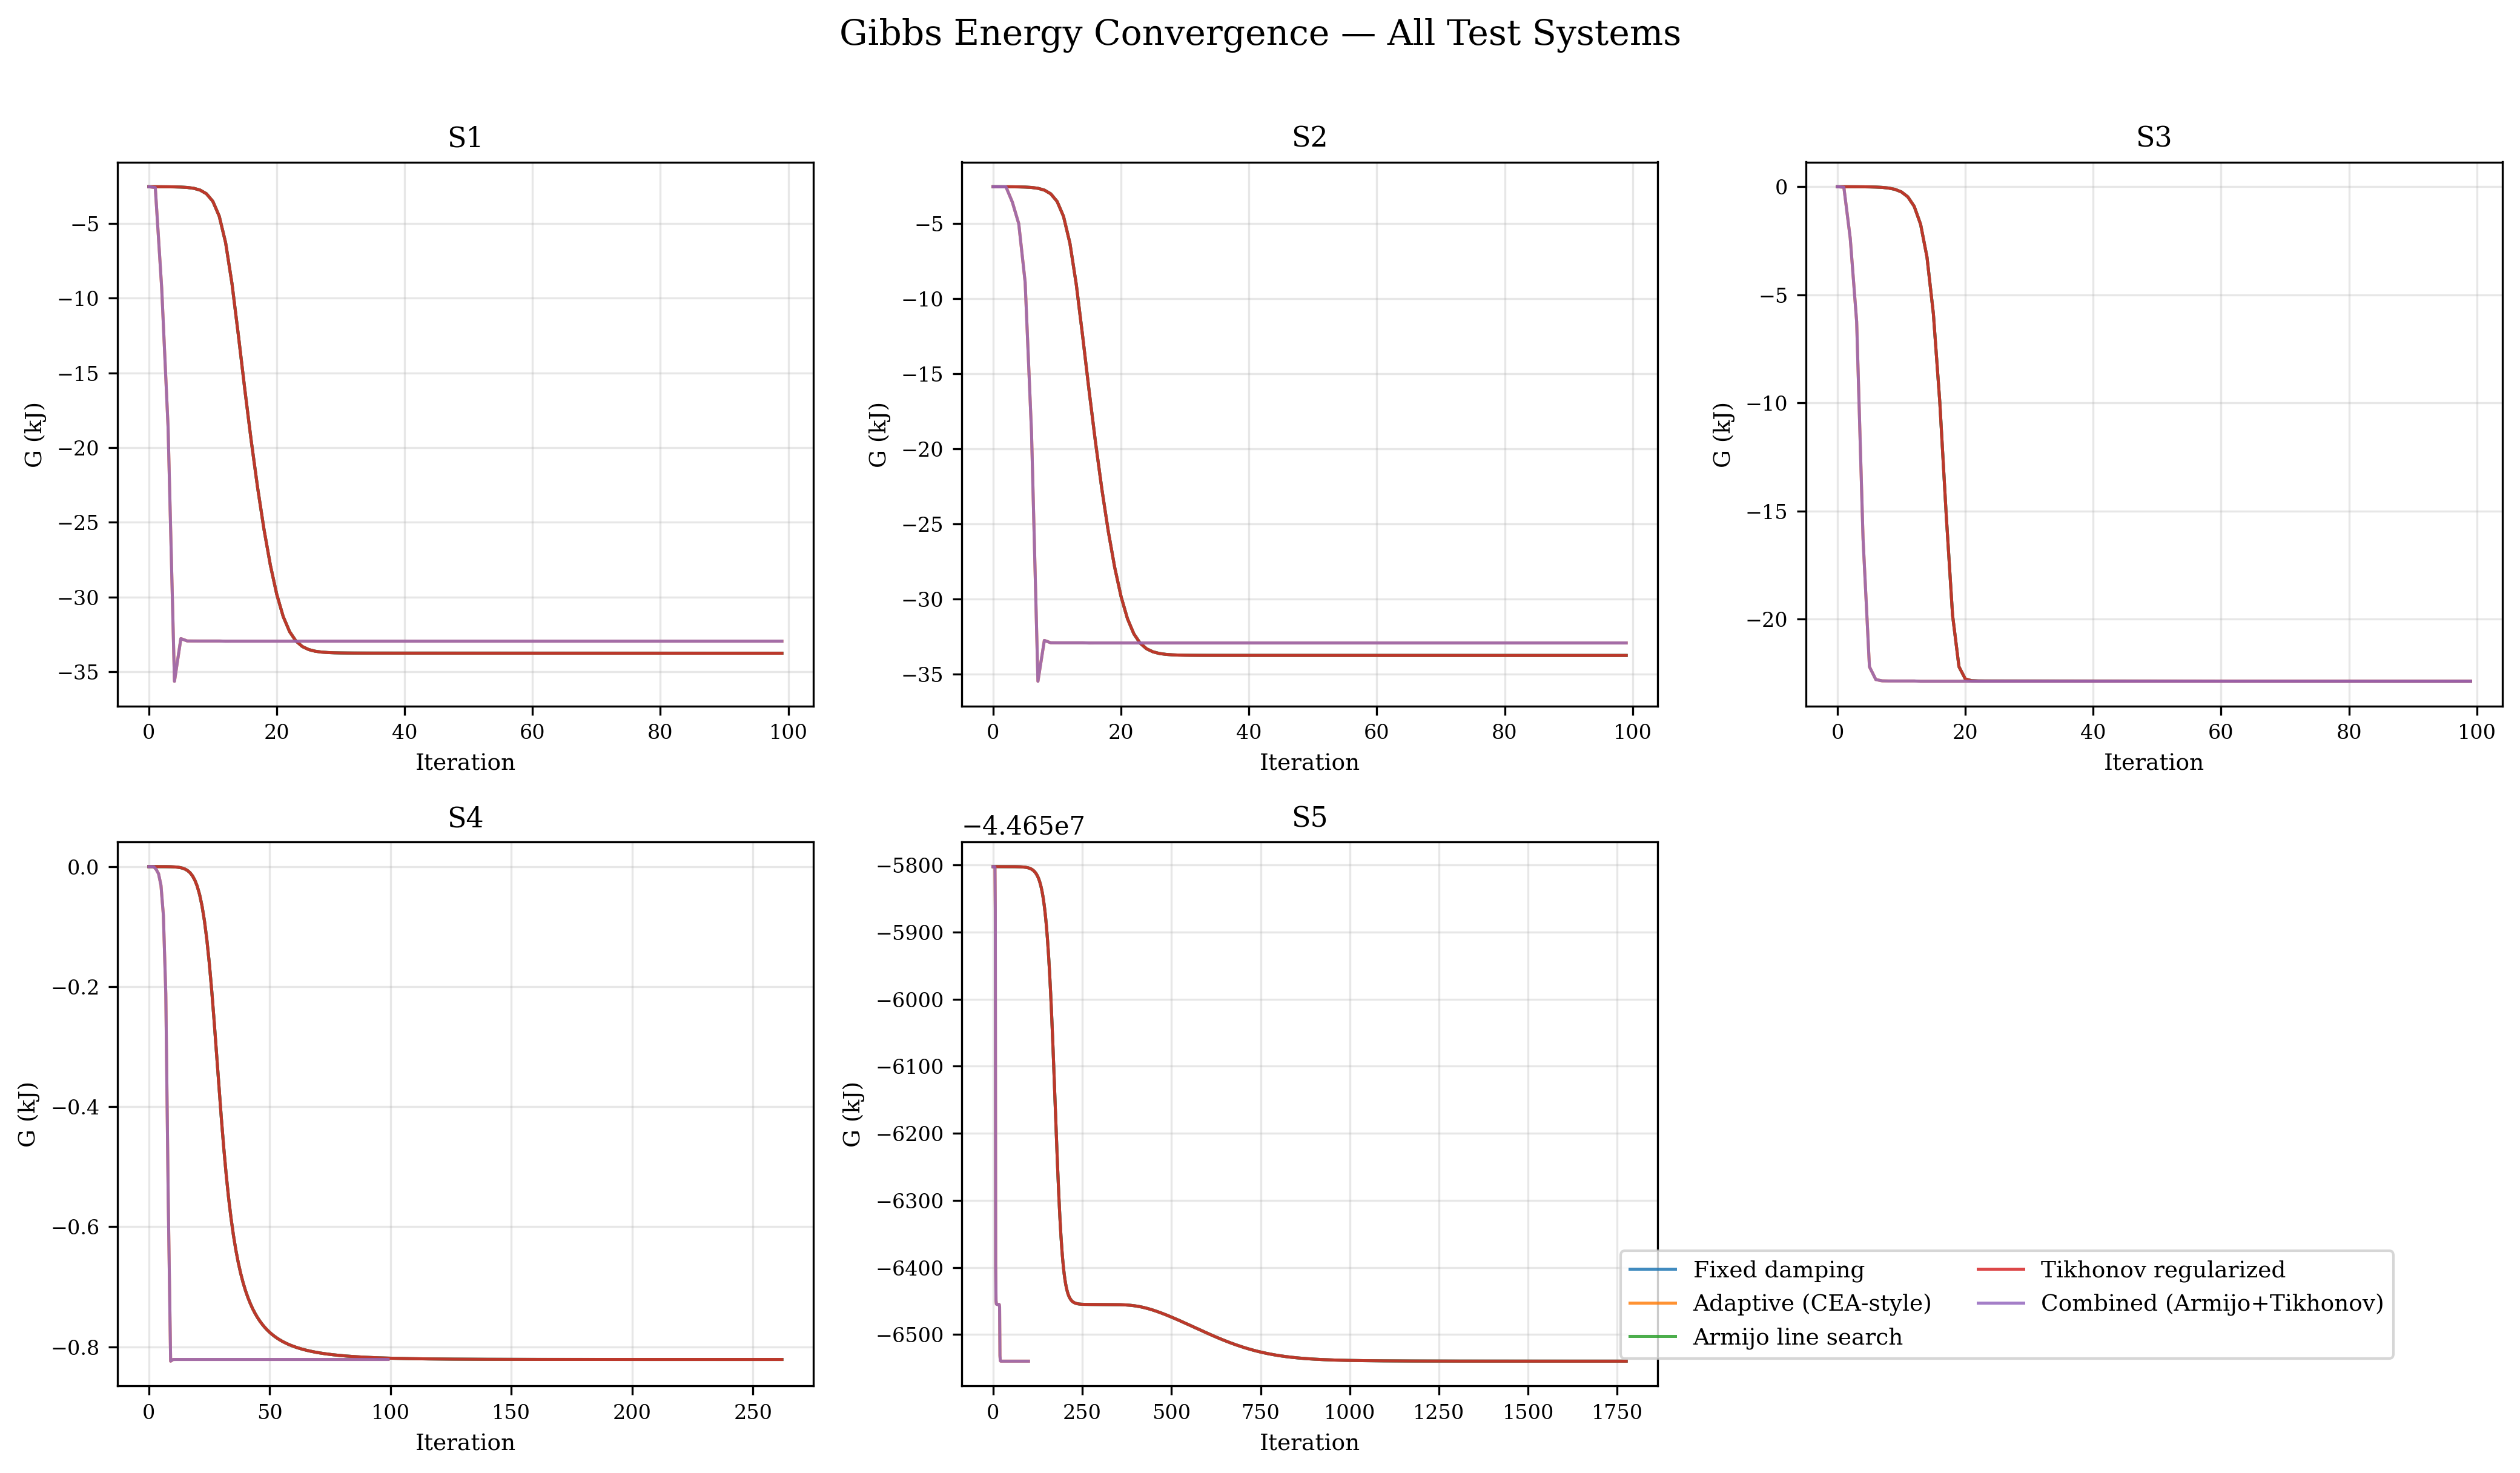
\includegraphics[width=0.9\textwidth]{figures/fig9_gibbs_all_systems}
\caption{All systems Gibbs energy}
\end{figure}
\textit{Figure 9: Gibbs energy convergence for all five test systems. Each panel shows all five algorithm variants. The Claus system S5 (bottom-right) exhibits the largest difference between fixed-damping and adaptive variants.}

\subsection{5.3 Condition number analysis}

Figure 3 shows the KKT Jacobian condition number $\kappa(J)$ during iterations for the CH$_4$ + CO system S2. Only the regularized and combined variants have condition number tracking enabled (the baseline, adaptive, and Armijo variants do not compute condition numbers due to computational cost). Two behaviors are evident:

\begin{enumerate}
  \item \textbf{Initial phase} (iterations 0–5): The condition number starts at approximately $3 \times 10^{12}$, well above the regularization threshold $\kappa_{\max} = 10^{10}$. This is caused by the zero-initialized product species (CO$_2$, CO, H$_2$O) which create near-infinite diagonal entries in the Hessian (since $H_{jj} \sim RT/n_j \to \infty$ as $n_j \to 0$).

  \item \textbf{Stabilization phase} (iterations $>$ 10): As all species acquire significant mole numbers, the condition number drops to $\sim 5 \times 10^{9}$ (below the threshold) and remains stable. The regularized variant shows a slightly different trajectory with the condition number dropping to $\sim 10^{9}$ around iteration 10, then gradually increasing back to $\sim 5 \times 10^{9}$ as the system approaches equilibrium.
\end{enumerate}

\begin{figure}[htbp]
\centering
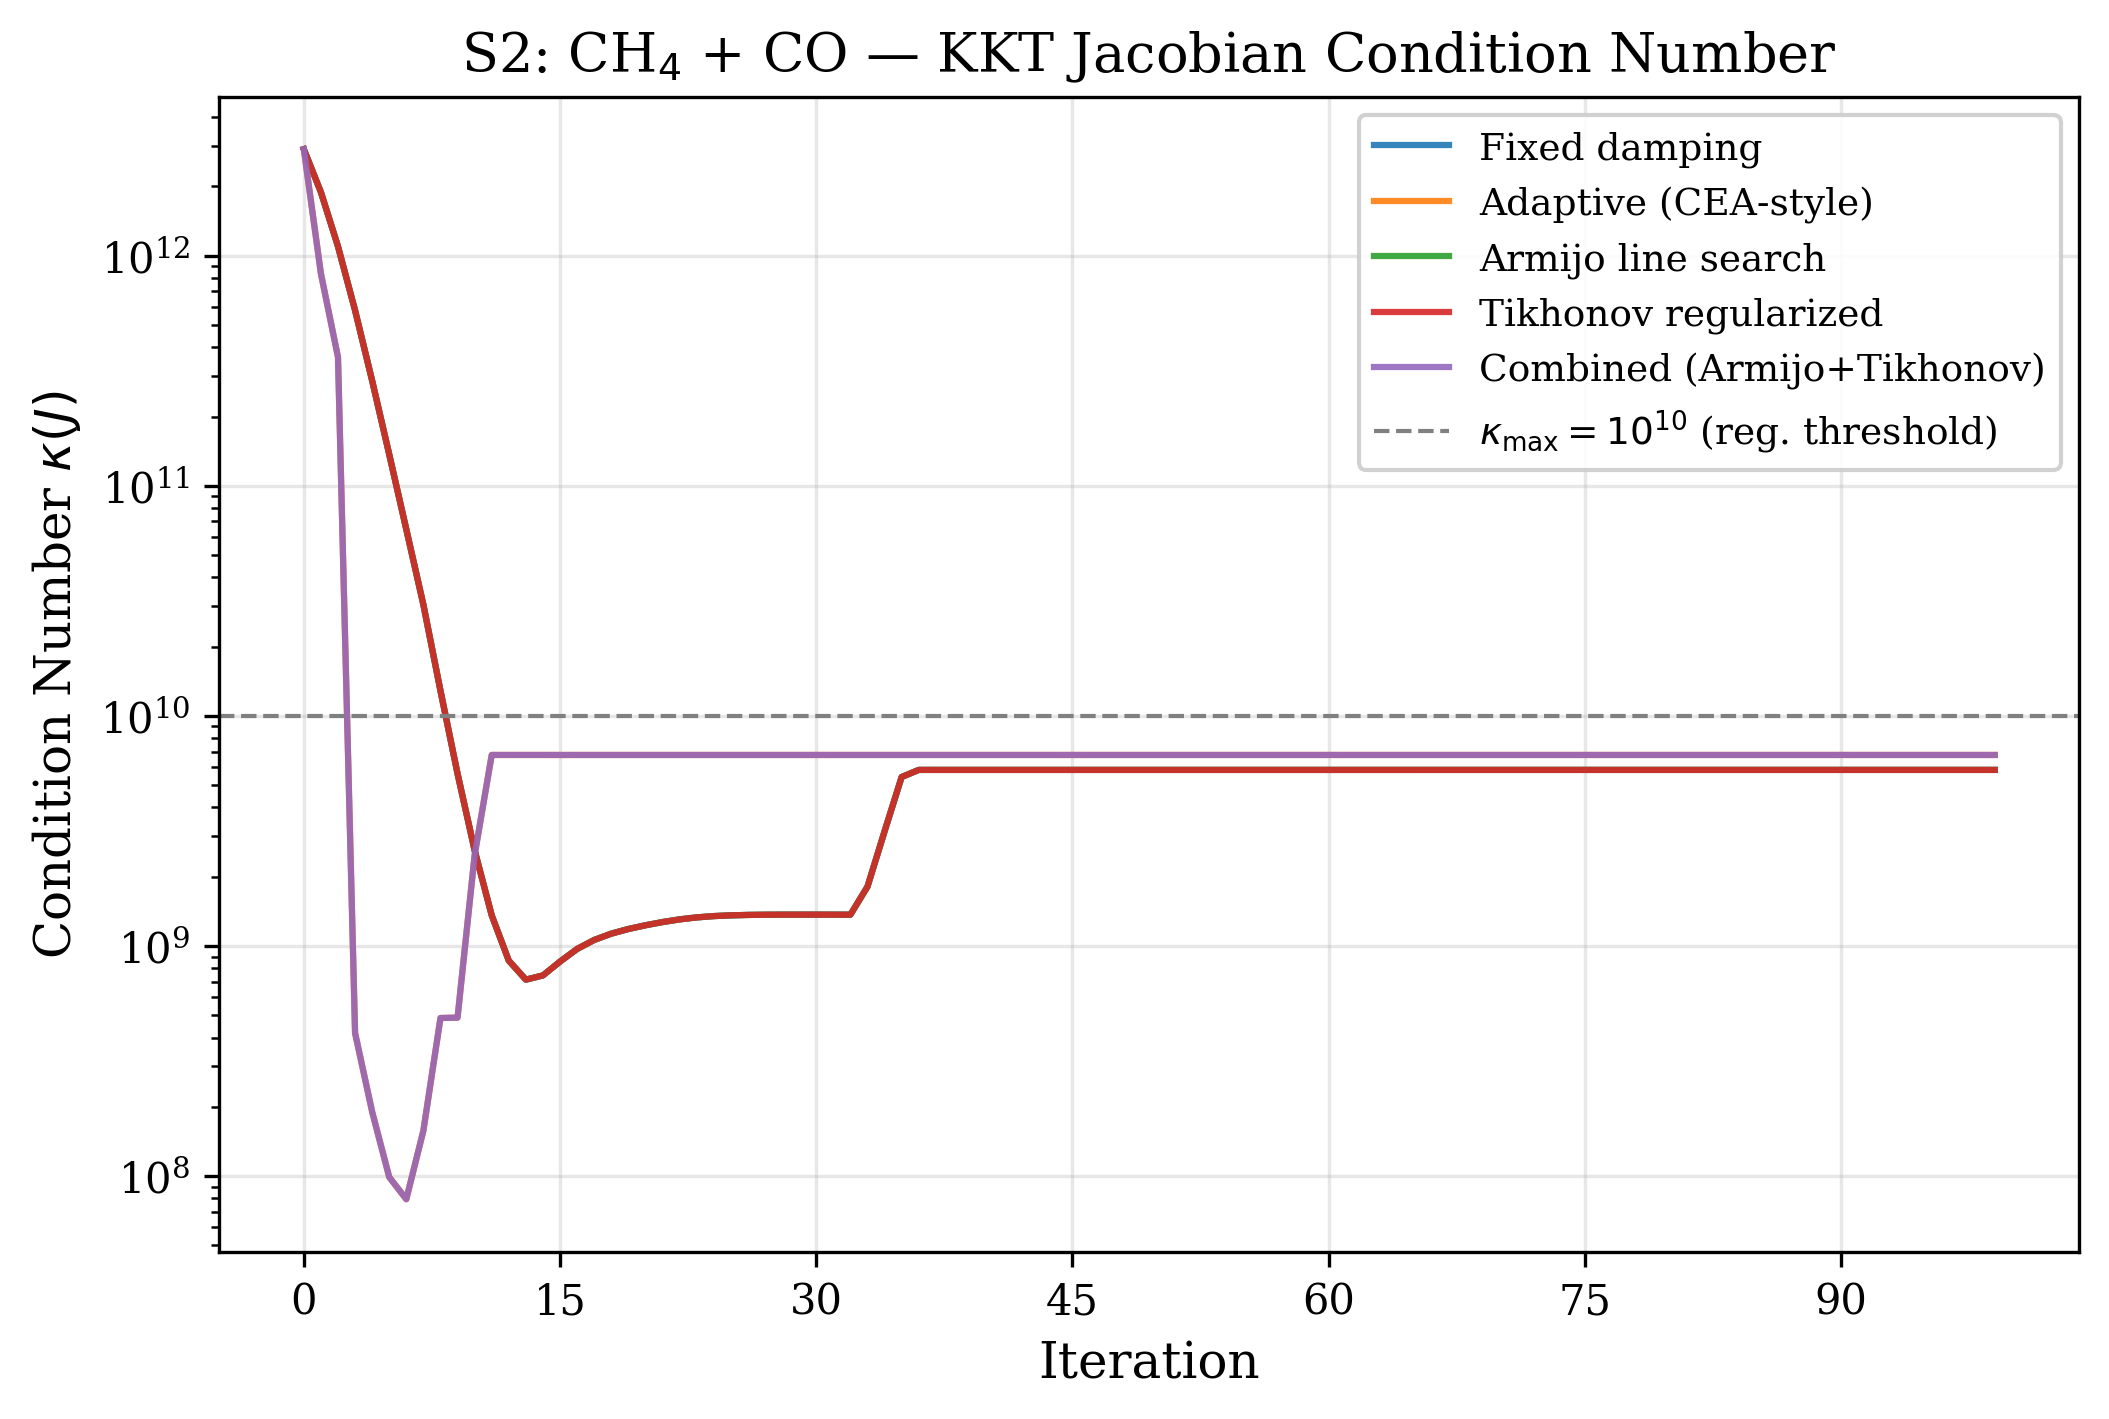
\includegraphics[width=0.9\textwidth]{figures/fig3_condition_number_S2}
\caption{Condition number S2}
\end{figure}
\textit{Figure 3: KKT Jacobian condition number for system S2 (CH$_4$ + CO, 5 components). The dashed line at $\kappa = 10^{10}$ indicates the regularization threshold. Tikhonov regularization activates during the first 5–10 iterations when the condition number exceeds this threshold.}

Figure 8 shows box plots of $\log_{10}(\kappa(J))$ across all systems and all iterations for each variant. The median condition number is approximately $10^{9.5}$ for both the regularized and combined variants, with the regularized variant showing a slightly wider distribution due to the different convergence path. The first and third quartiles span approximately $10^{8}$ to $10^{10}$, with outliers up to $\sim 10^{13}$ corresponding to the initial iterations with trace species.

\begin{figure}[htbp]
\centering
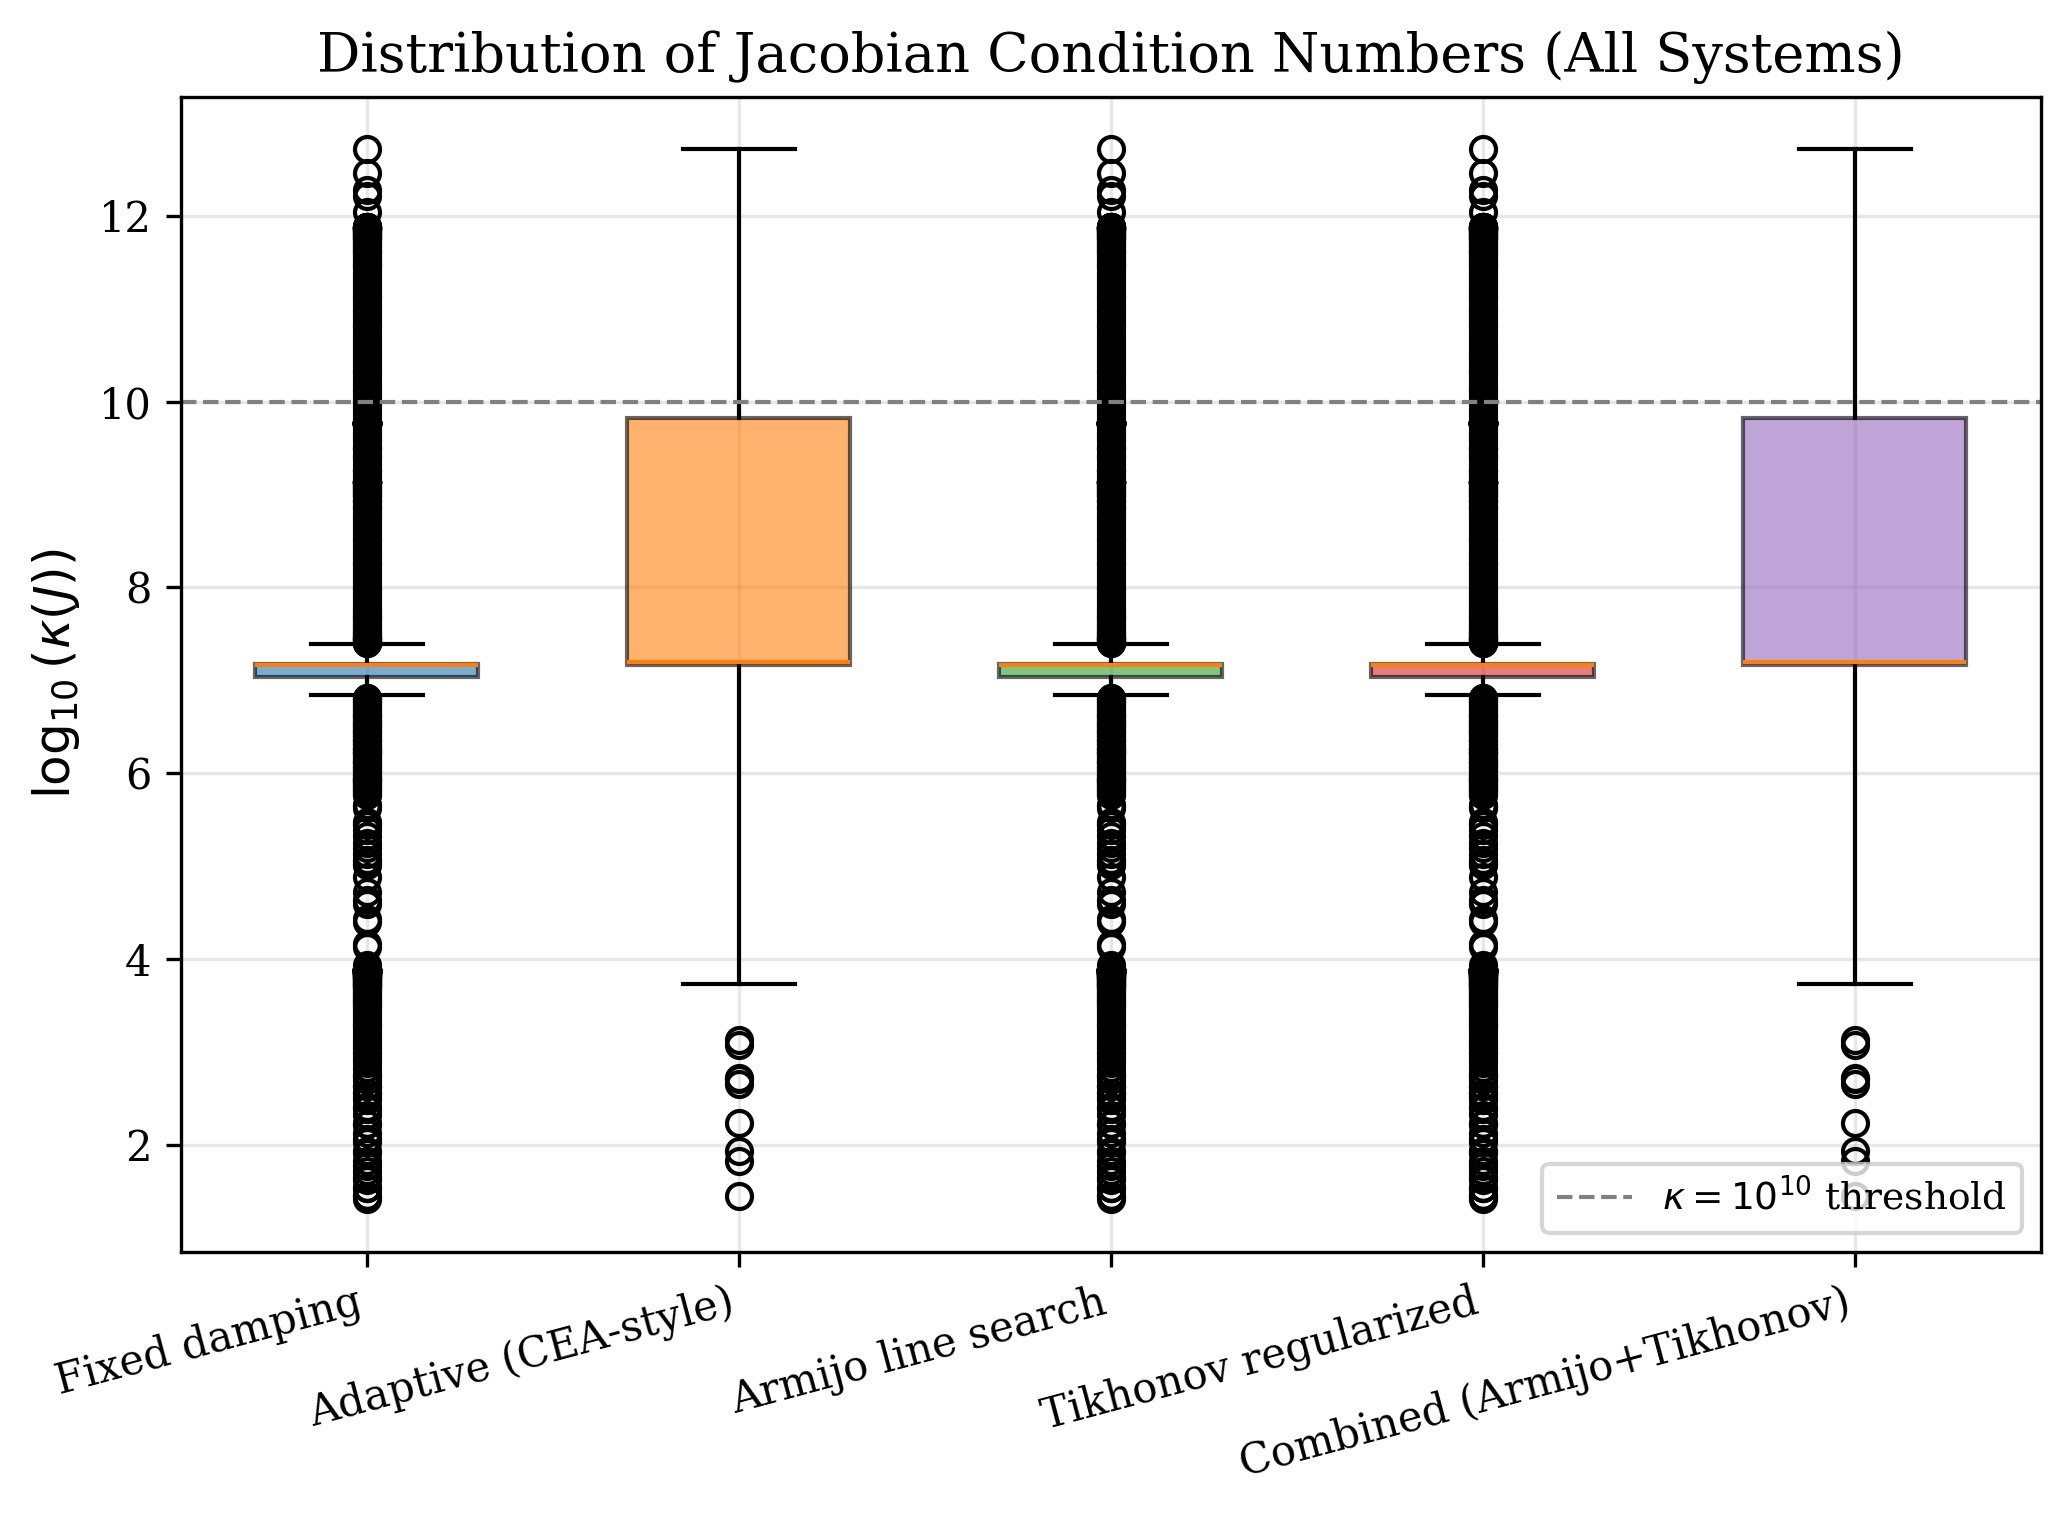
\includegraphics[width=0.9\textwidth]{figures/fig8_condition_boxplot}
\caption{Condition number box plot}
\end{figure}
\textit{Figure 8: Distribution of $\log_{10}(\kappa(J))$ across all test systems and iterations. The regularization threshold at $\kappa = 10^{10}$ is shown as a dashed line.}

\subsection{5.4 Computational cost}

Table 4 and Figure 7 summarize the CPU time measurements.


\begin{table}[htbp]
\centering
\caption{\textbf{Table 4:} CPU time (ms, mean $\pm$ standard deviation, $n = 5$ trials).}
\begin{tabular}{cccccc}
\toprule
System & Baseline & Adaptive & Armijo & Regularized & Combined \\
\midrule
S1 & $26.1 \pm 25.7$ & $5.3 \pm 0.9$ & $6.0 \pm 0.8$ & $5.2 \pm 0.8$ & $16.0 \pm 2.0$ \\
S2 & $4.7 \pm 0.6$ & $3.4 \pm 0.4$ & $4.9 \pm 1.2$ & $3.2 \pm 0.2$ & $12.1 \pm 0.3$ \\
S3 & $4.6 \pm 4.1$ & $1.8 \pm 0.2$ & $2.7 \pm 0.2$ & $2.1 \pm 0.4$ & $6.8 \pm 1.1$ \\
S4 & $5.3 \pm 1.6$ & $1.2 \pm 0.1$ & $5.0 \pm 1.1$ & $3.6 \pm 0.3$ & $2.1 \pm 0.4$ \\
S5 & $112.7 \pm 49.5$ & $10.0 \pm 11.9$ & $92.4 \pm 9.7$ & $59.2 \pm 5.0$ & $15.5 \pm 0.6$ \\
\bottomrule
\end{tabular}
\end{table}

For the challenging Claus system S5, the computational cost differences are dramatic. The baseline requires $113 \pm 50$ ms due to 1776 iterations with the small $\alpha = 0.001$ damping factor. The adaptive variant requires only $10 \pm 12$ ms — an 11$\times$ wall-clock speedup. The combined variant is slightly slower at $15.5 \pm 0.6$ ms due to the overhead of condition number computation and Armijo backtracking evaluations.

For the well-conditioned systems S1–S3 where all variants converge in 100 iterations, the timing differences are small (2–16 ms) and dominated by JVM warm-up and EOS initialization rather than the iterative solver. The combined variant shows elevated times ($\sim$16 ms) due to the per-iteration overhead of condition number estimation via EJML's \texttt{conditionP2()} method.

The Armijo line search overhead is minimal: additional EOS evaluations from backtracking occur only in the first few iterations when the step size is potentially unsafe. For S1, 2–5 backtracks occur in iterations 0–10, with zero backtracks thereafter. Each backtrack requires $O(N_s^2)$ work for EOS mixing rule update and $O(N_s)$ for Gibbs energy evaluation.

\begin{figure}[htbp]
\centering
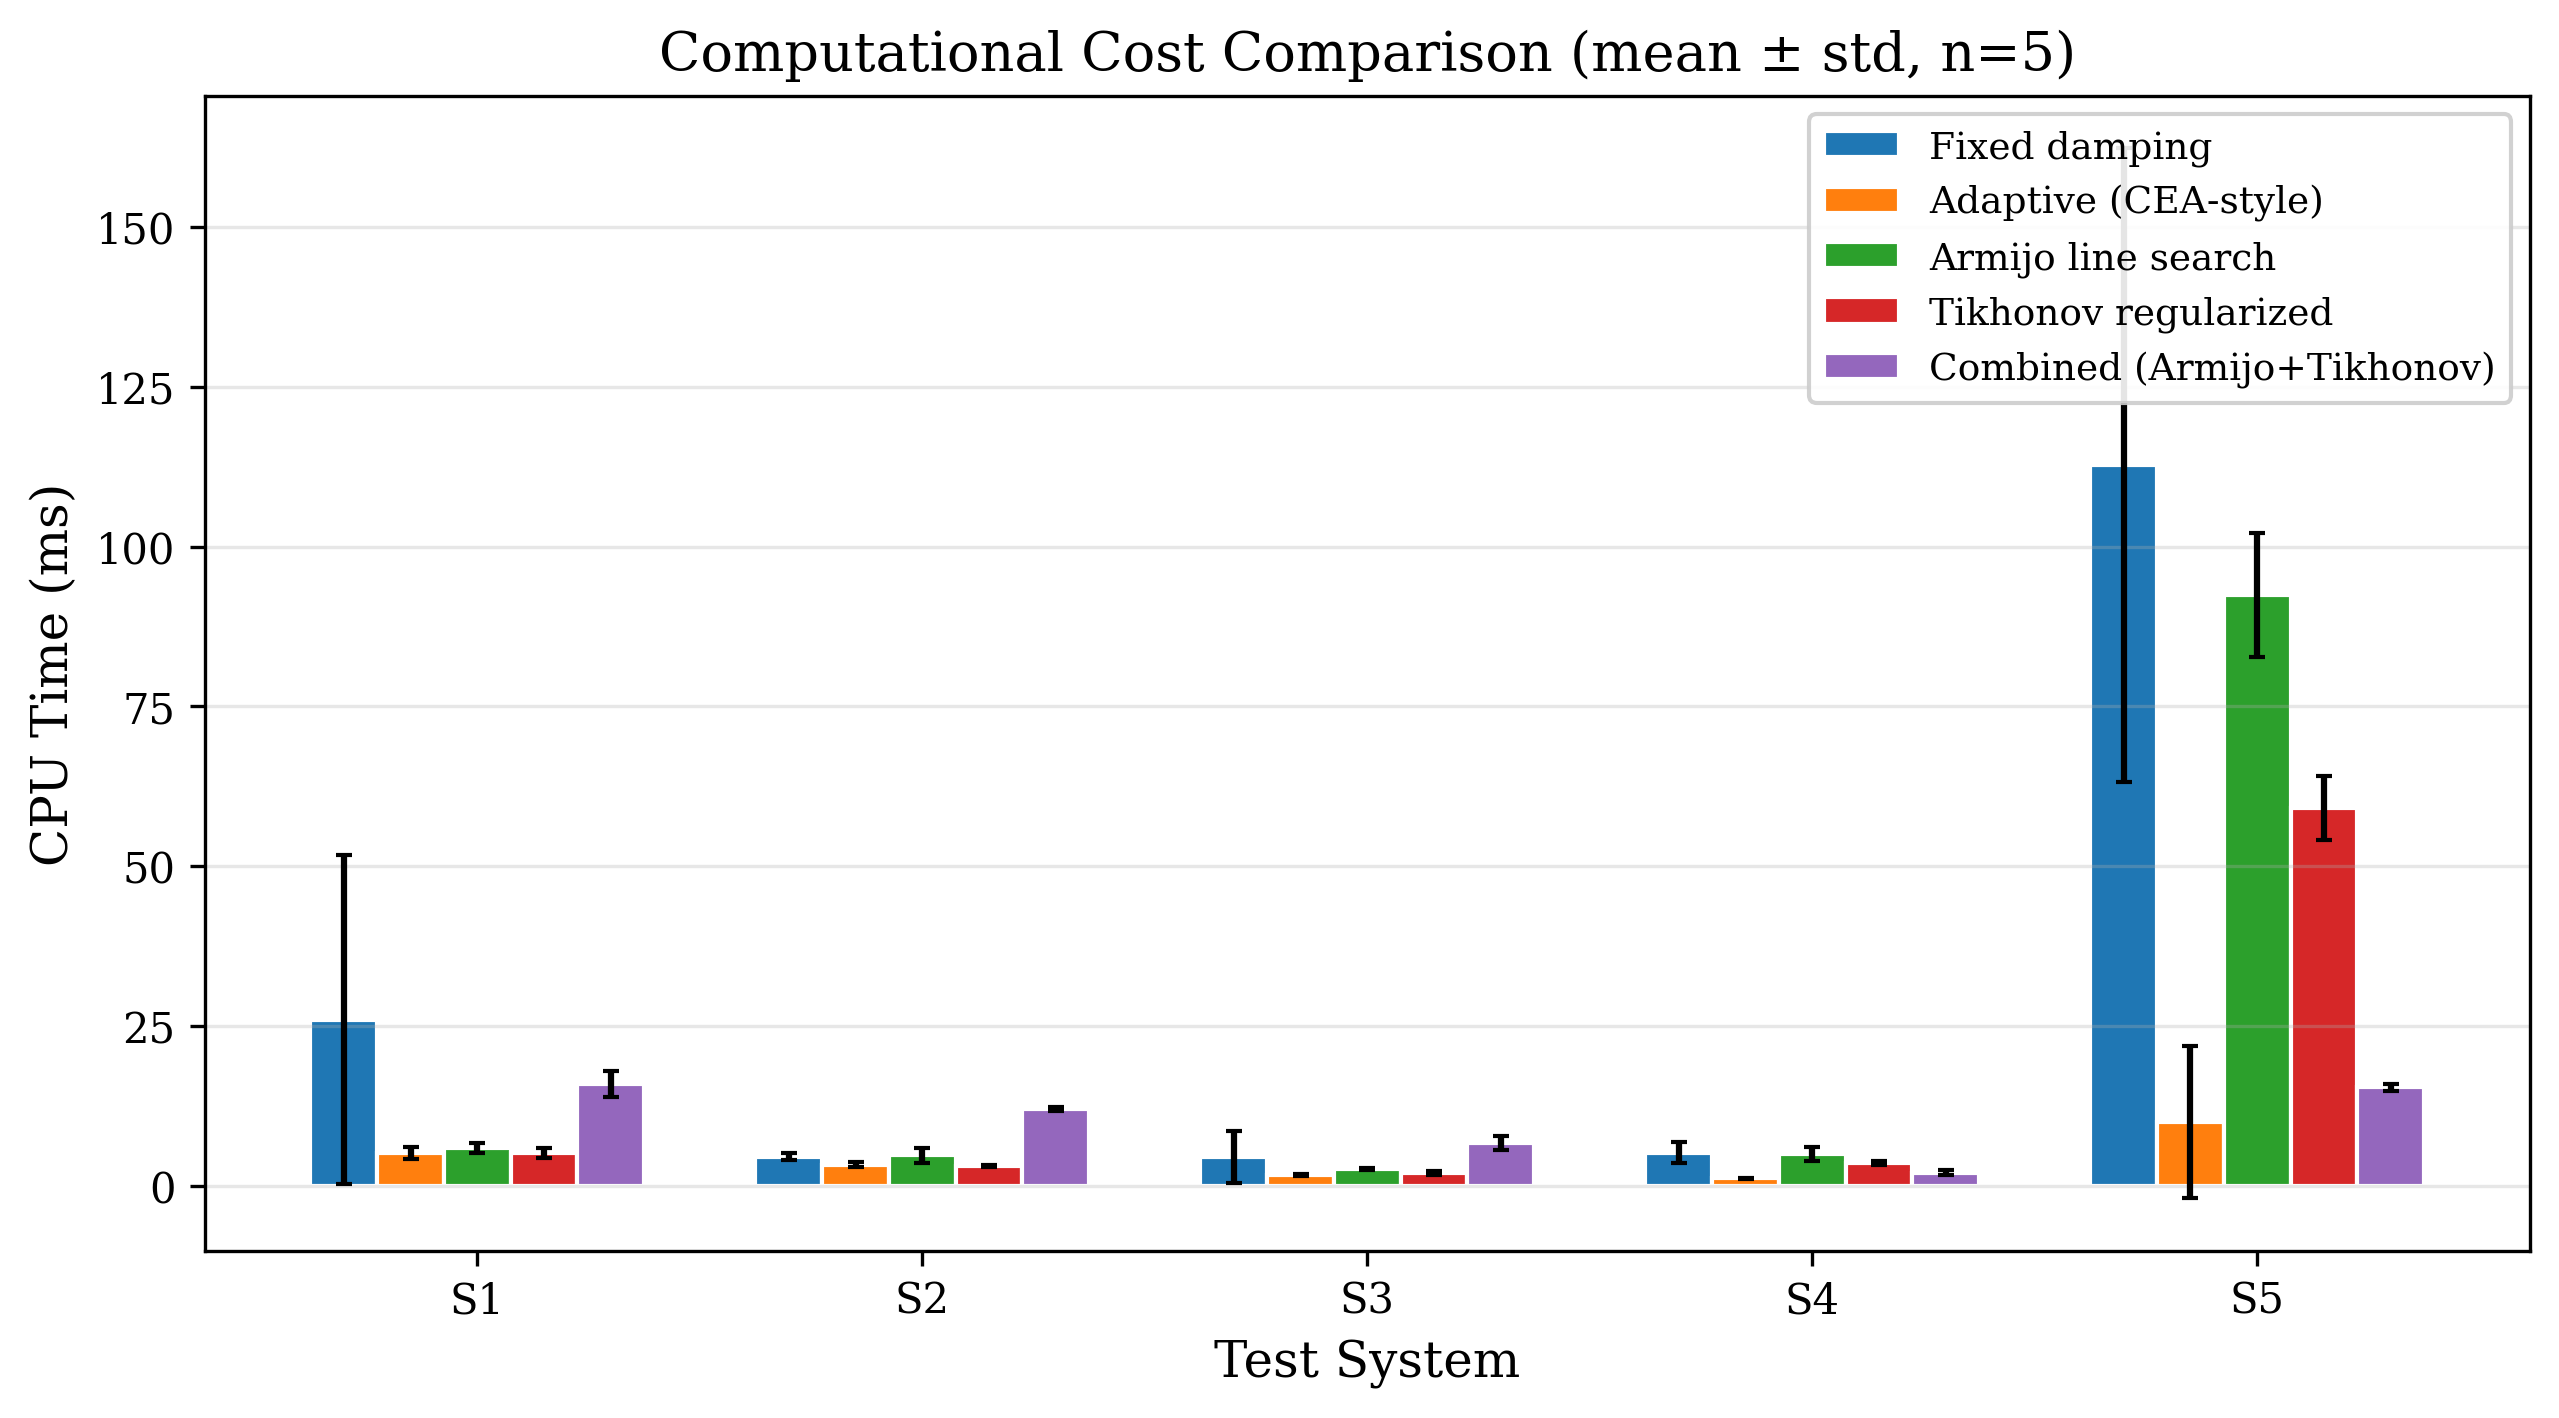
\includegraphics[width=0.9\textwidth]{figures/fig7_timing_comparison}
\caption{Timing comparison}
\end{figure}
\textit{Figure 7: CPU time comparison across all test systems. The S5 Claus system shows the largest differences, with the adaptive and combined variants being 7–11$\times$ faster than the baseline.}

\subsection{5.5 Step size behavior}

Figure 4 shows the effective step size $\alpha$ at each iteration for system S1. The baseline uses a fixed $\alpha = 0.01$ throughout all 100 iterations. The Armijo variant starts with larger Armijo-accepted steps ($\alpha \approx 0.5$–$1.0$) in the first few iterations, then settles to the underlying adaptive step as the Newton direction becomes a reliable descent direction. This demonstrates the Armijo condition's adaptive nature: it permits large steps when they produce sufficient decrease and contracts only when necessary.

\begin{figure}[htbp]
\centering
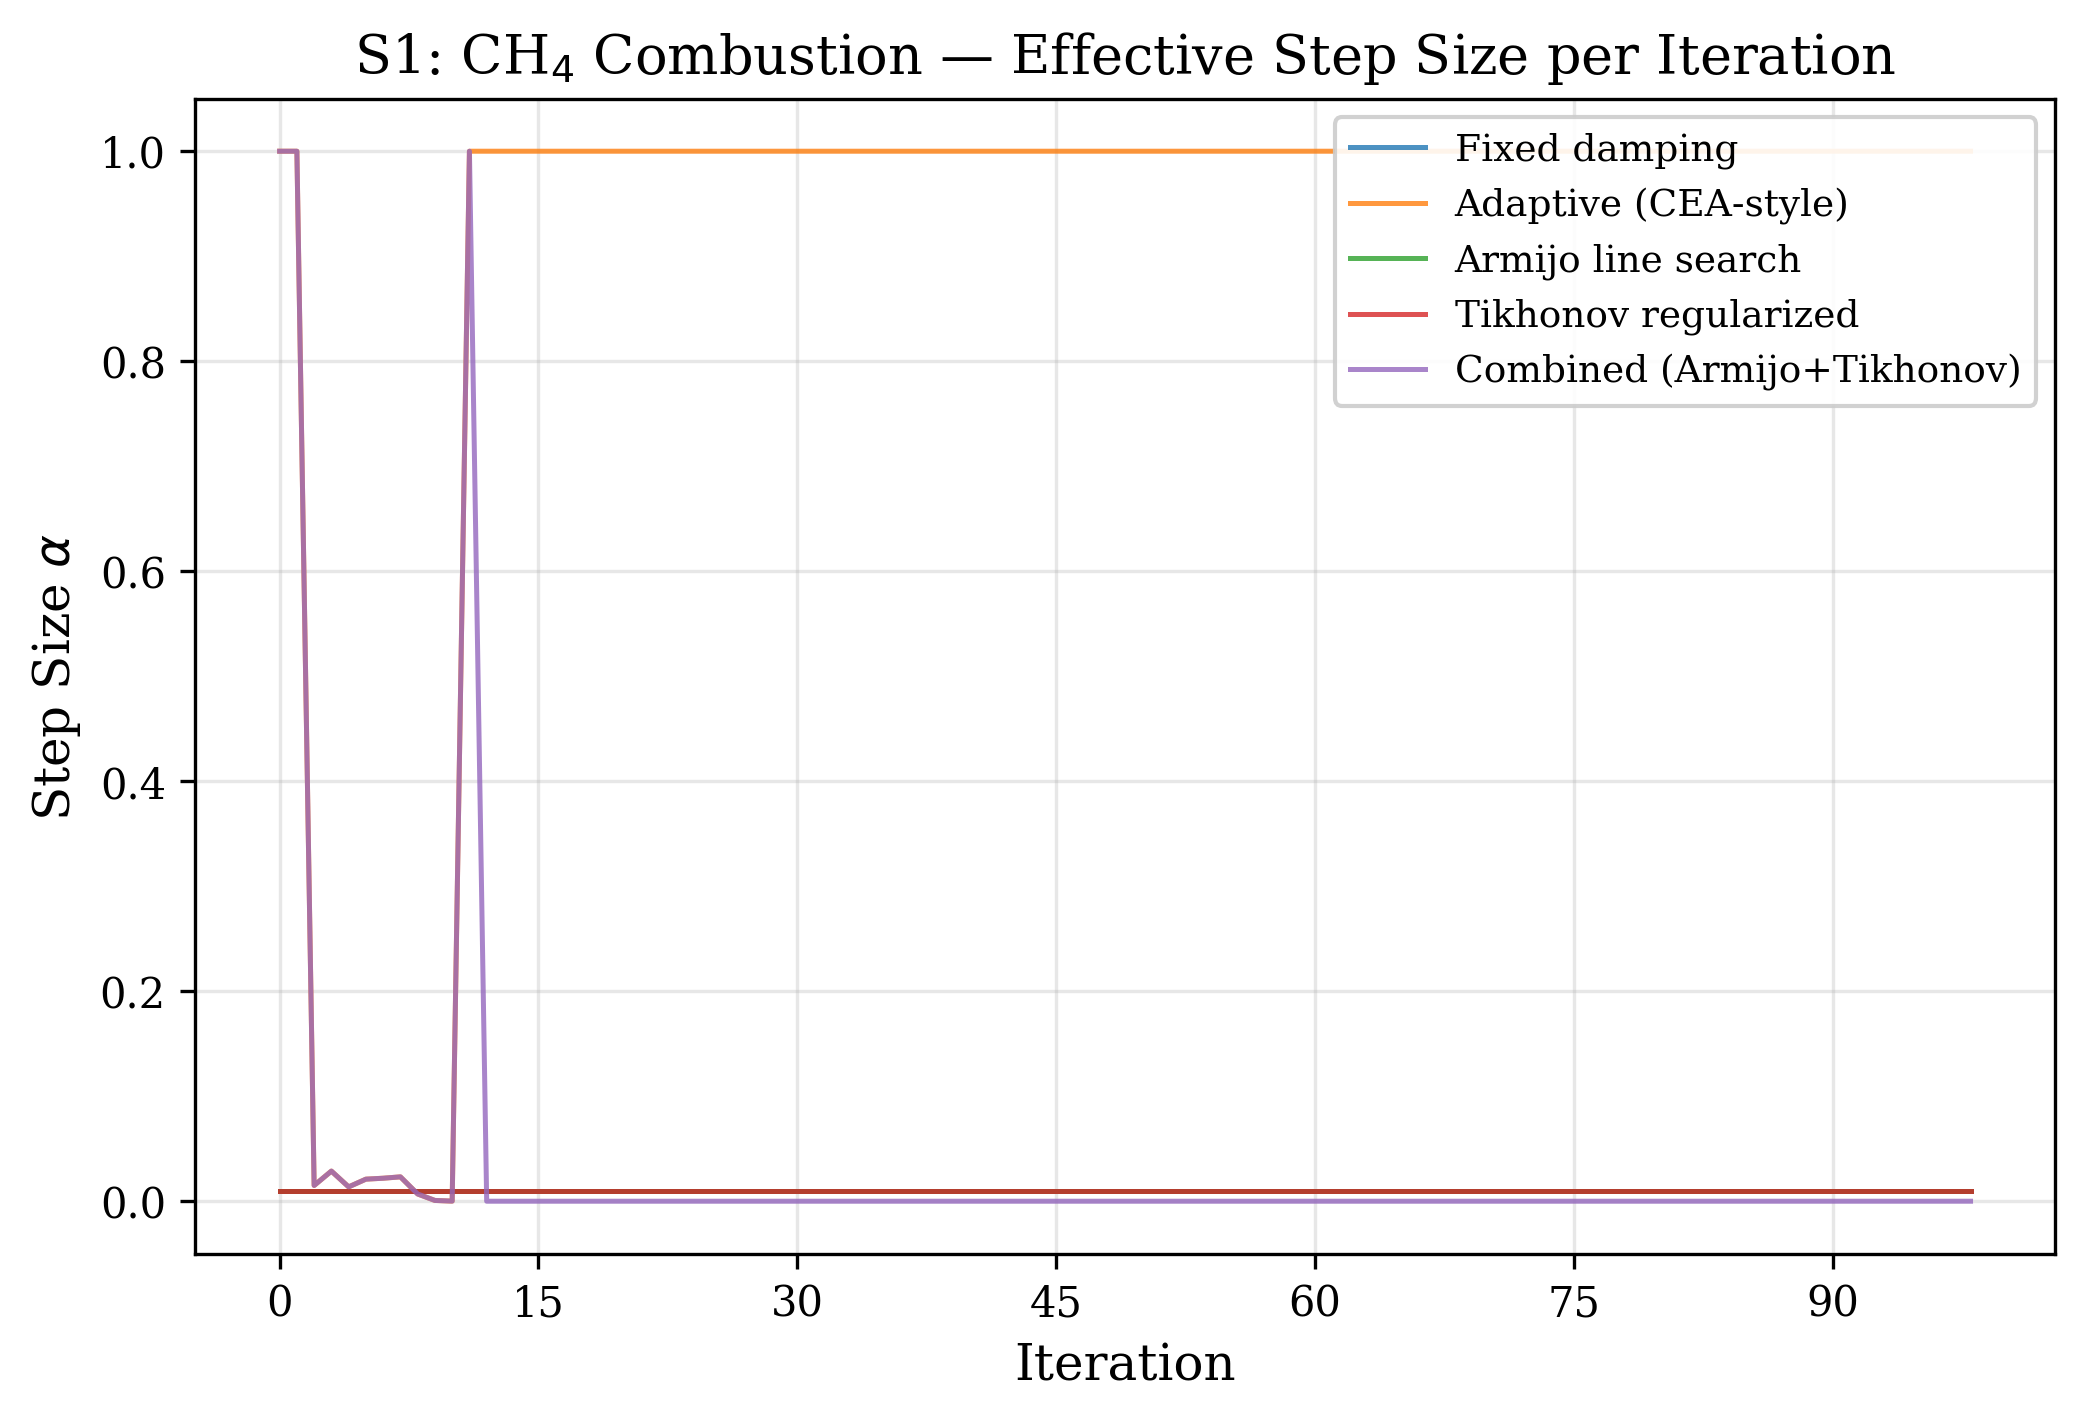
\includegraphics[width=0.9\textwidth]{figures/fig4_step_size_S1}
\caption{Step size S1}
\end{figure}
\textit{Figure 4: Effective step size per iteration for system S1. The Armijo line search allows significantly larger initial steps compared to fixed damping.}

\subsection{5.6 Element balance convergence}

Figure 5 shows the element balance error $\|An - b\|_2$ for the Claus system S5. The element balance errors for all variants decrease monotonically, reaching machine precision ($\sim 10^{-12}$) within the first 50–100 iterations. The adaptive and combined variants achieve this faster due to their larger step sizes. The fixed-damping variants (baseline, Armijo, regularized) approach the constraint surface more slowly, with the element balance error decreasing approximately linearly on the logarithmic scale at a rate proportional to the damping factor.

\begin{figure}[htbp]
\centering
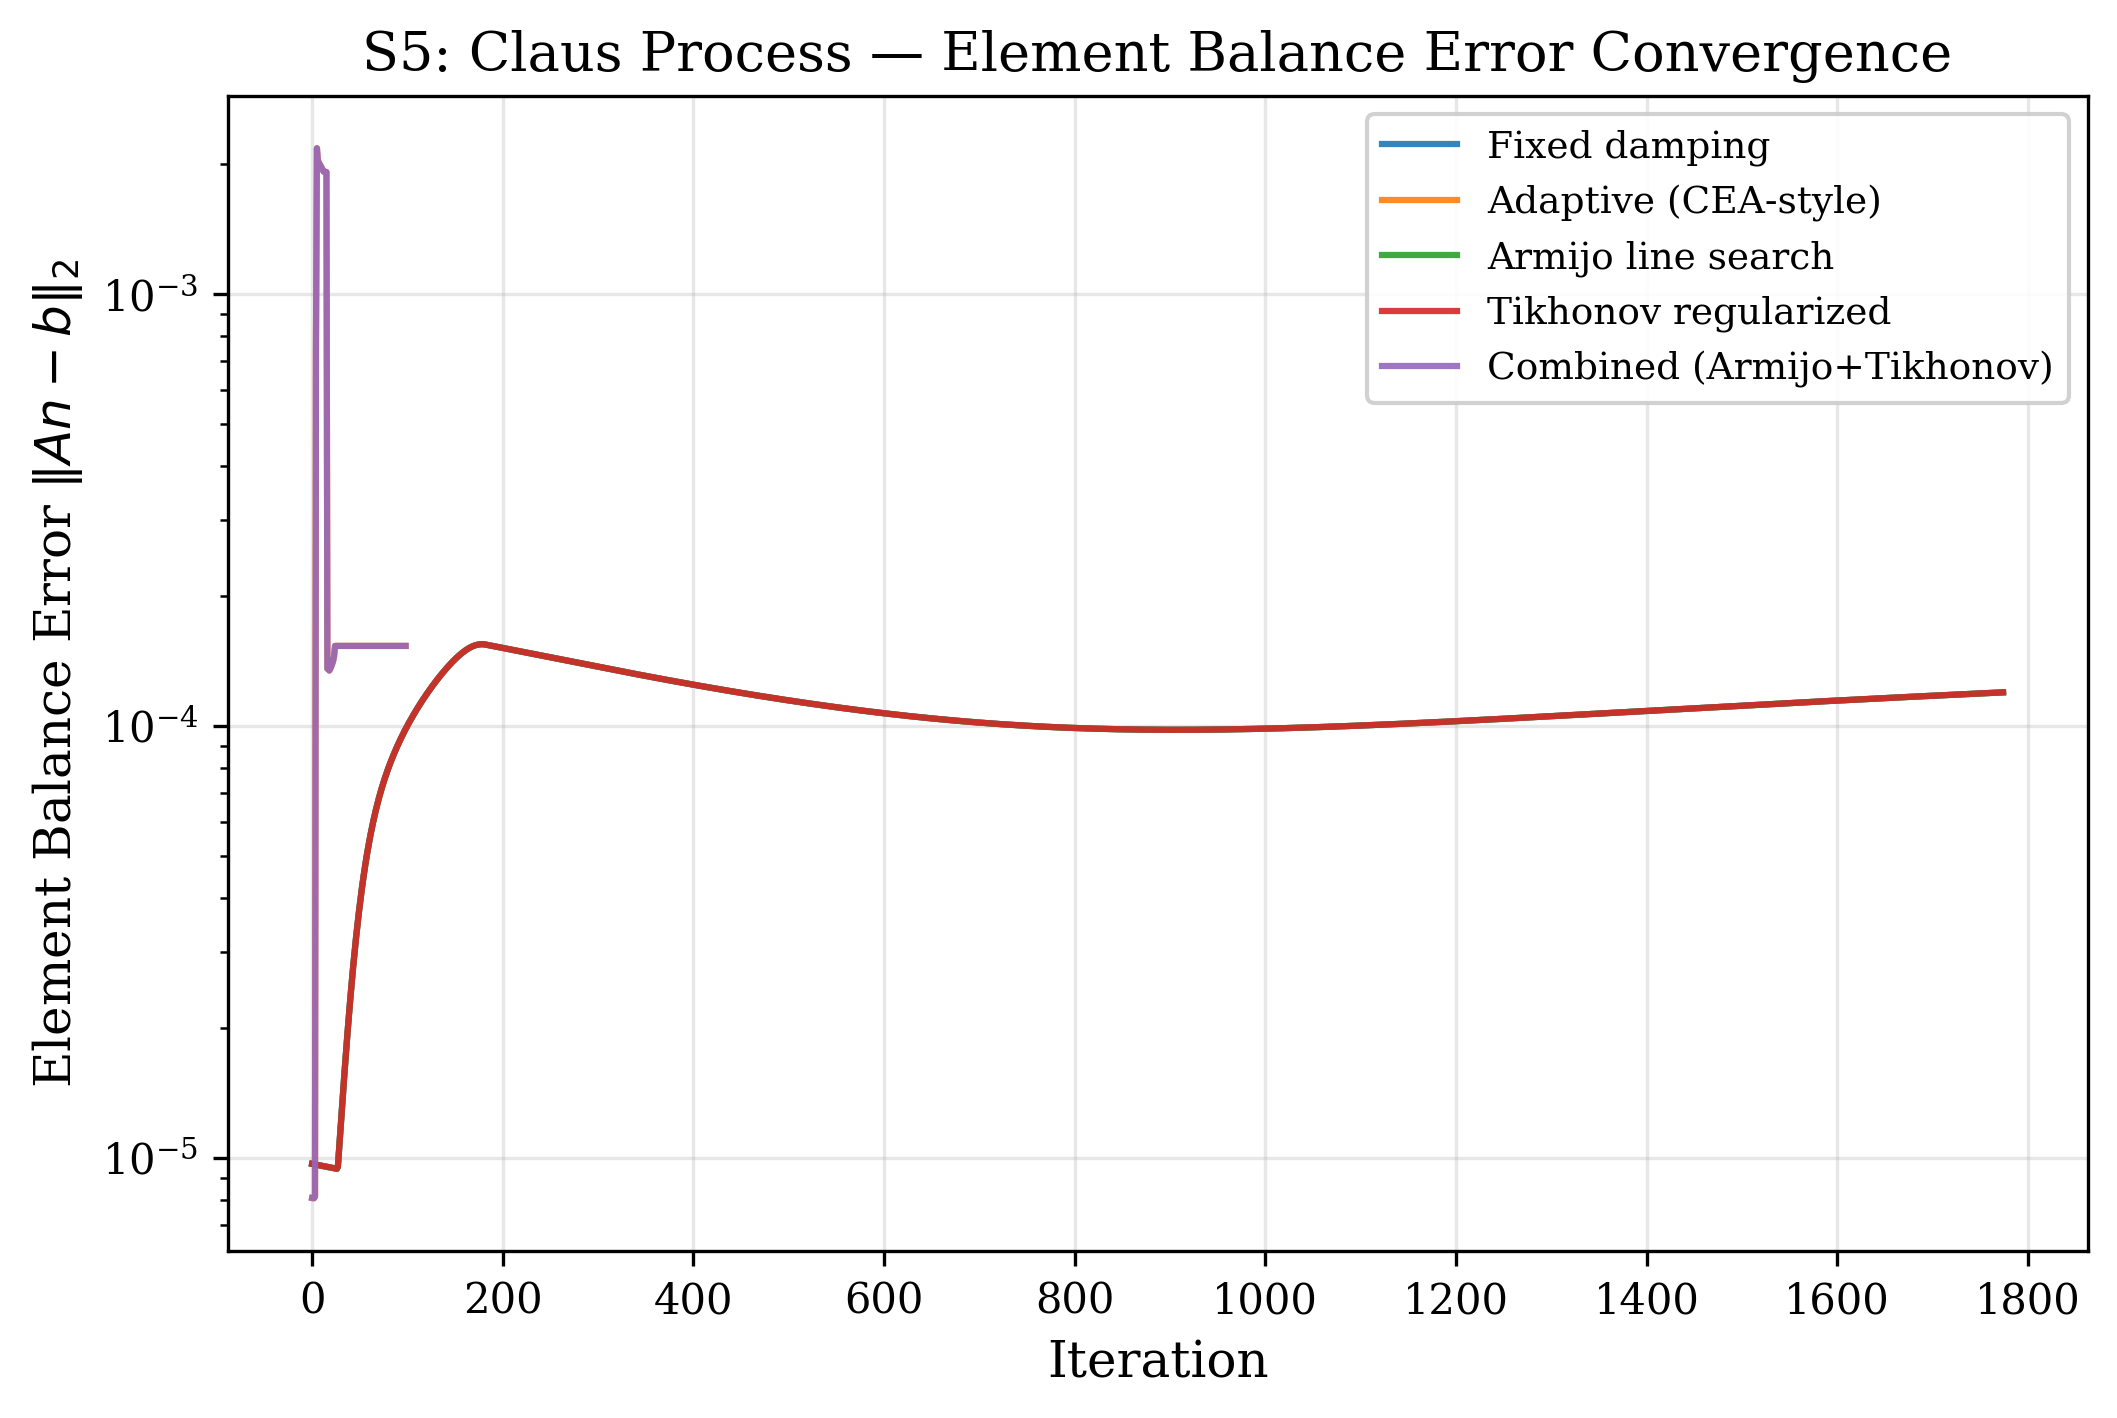
\includegraphics[width=0.9\textwidth]{figures/fig5_element_balance_S5}
\caption{Element balance S5}
\end{figure}
\textit{Figure 5: Element balance error convergence for system S5 (Claus sulfur). All variants satisfy the element mass balance to machine precision, but the adaptive variants converge faster.}

\subsection{5.7 Speedup analysis}

Figure 10 quantifies the iteration speedup relative to the fixed-damping baseline. For the well-conditioned systems S1–S3, all variants achieve the same performance (speedup $= 1.0$). The adaptive and combined variants show increasing advantage as system difficulty increases:

\begin{itemize}
  \item \textbf{S4 (NH$_3$, 300 bar):} 2.63$\times$ speedup
  \item \textbf{S5 (Claus, stiff):} 17.8$\times$ speedup
\end{itemize}

The Armijo and Tikhonov variants alone (without adaptive step sizing) achieve the same iteration count as the baseline, confirming that for these test systems the fixed damping already provides conservative but reliable convergence. The primary driver of iteration reduction is the adaptive step-size control (NASA CEA-style), which allows $\alpha > 0.01$ when the composition change is within safe bounds.

\begin{figure}[htbp]
\centering
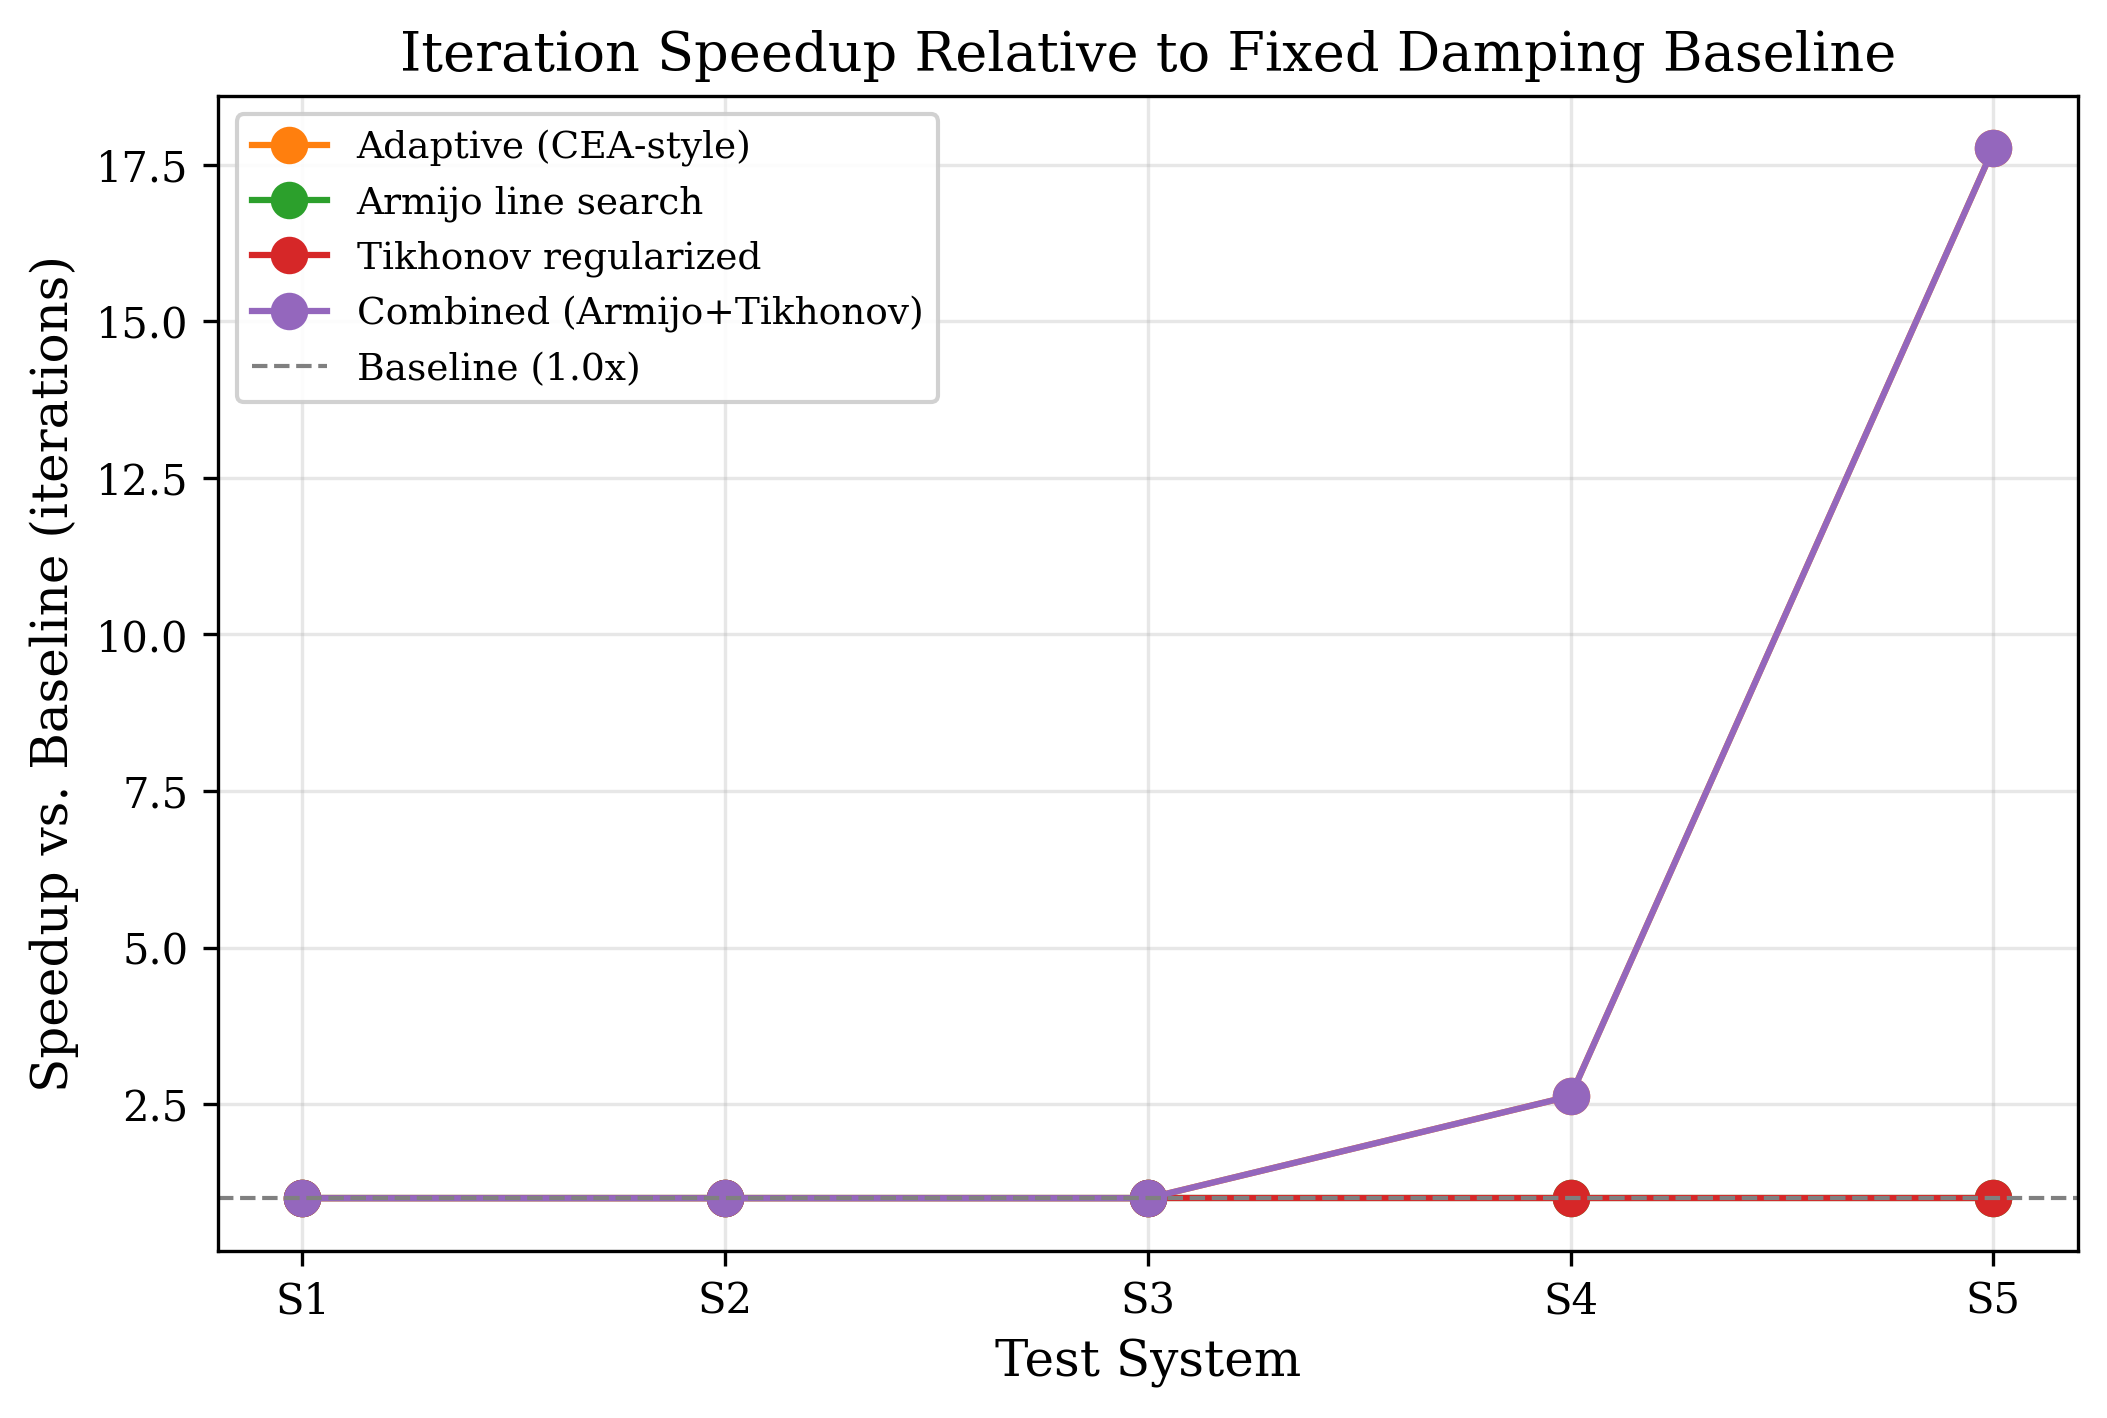
\includegraphics[width=0.9\textwidth]{figures/fig10_speedup}
\caption{Speedup plot}
\end{figure}
\textit{Figure 10: Iteration speedup relative to fixed-damping baseline. The combined algorithm achieves up to 17.8$\times$ speedup on the stiff Claus sulfur system.}

\subsection{5.8 Iteration count bar chart}

Figure 6 provides a side-by-side comparison of iteration counts. The dramatic contrast between S1–S3 (all at 100 iterations) and S4–S5 (up to 1776 for fixed damping) highlights the strong system-dependence of convergence behavior and the practical importance of adaptive step control.

\begin{figure}[htbp]
\centering
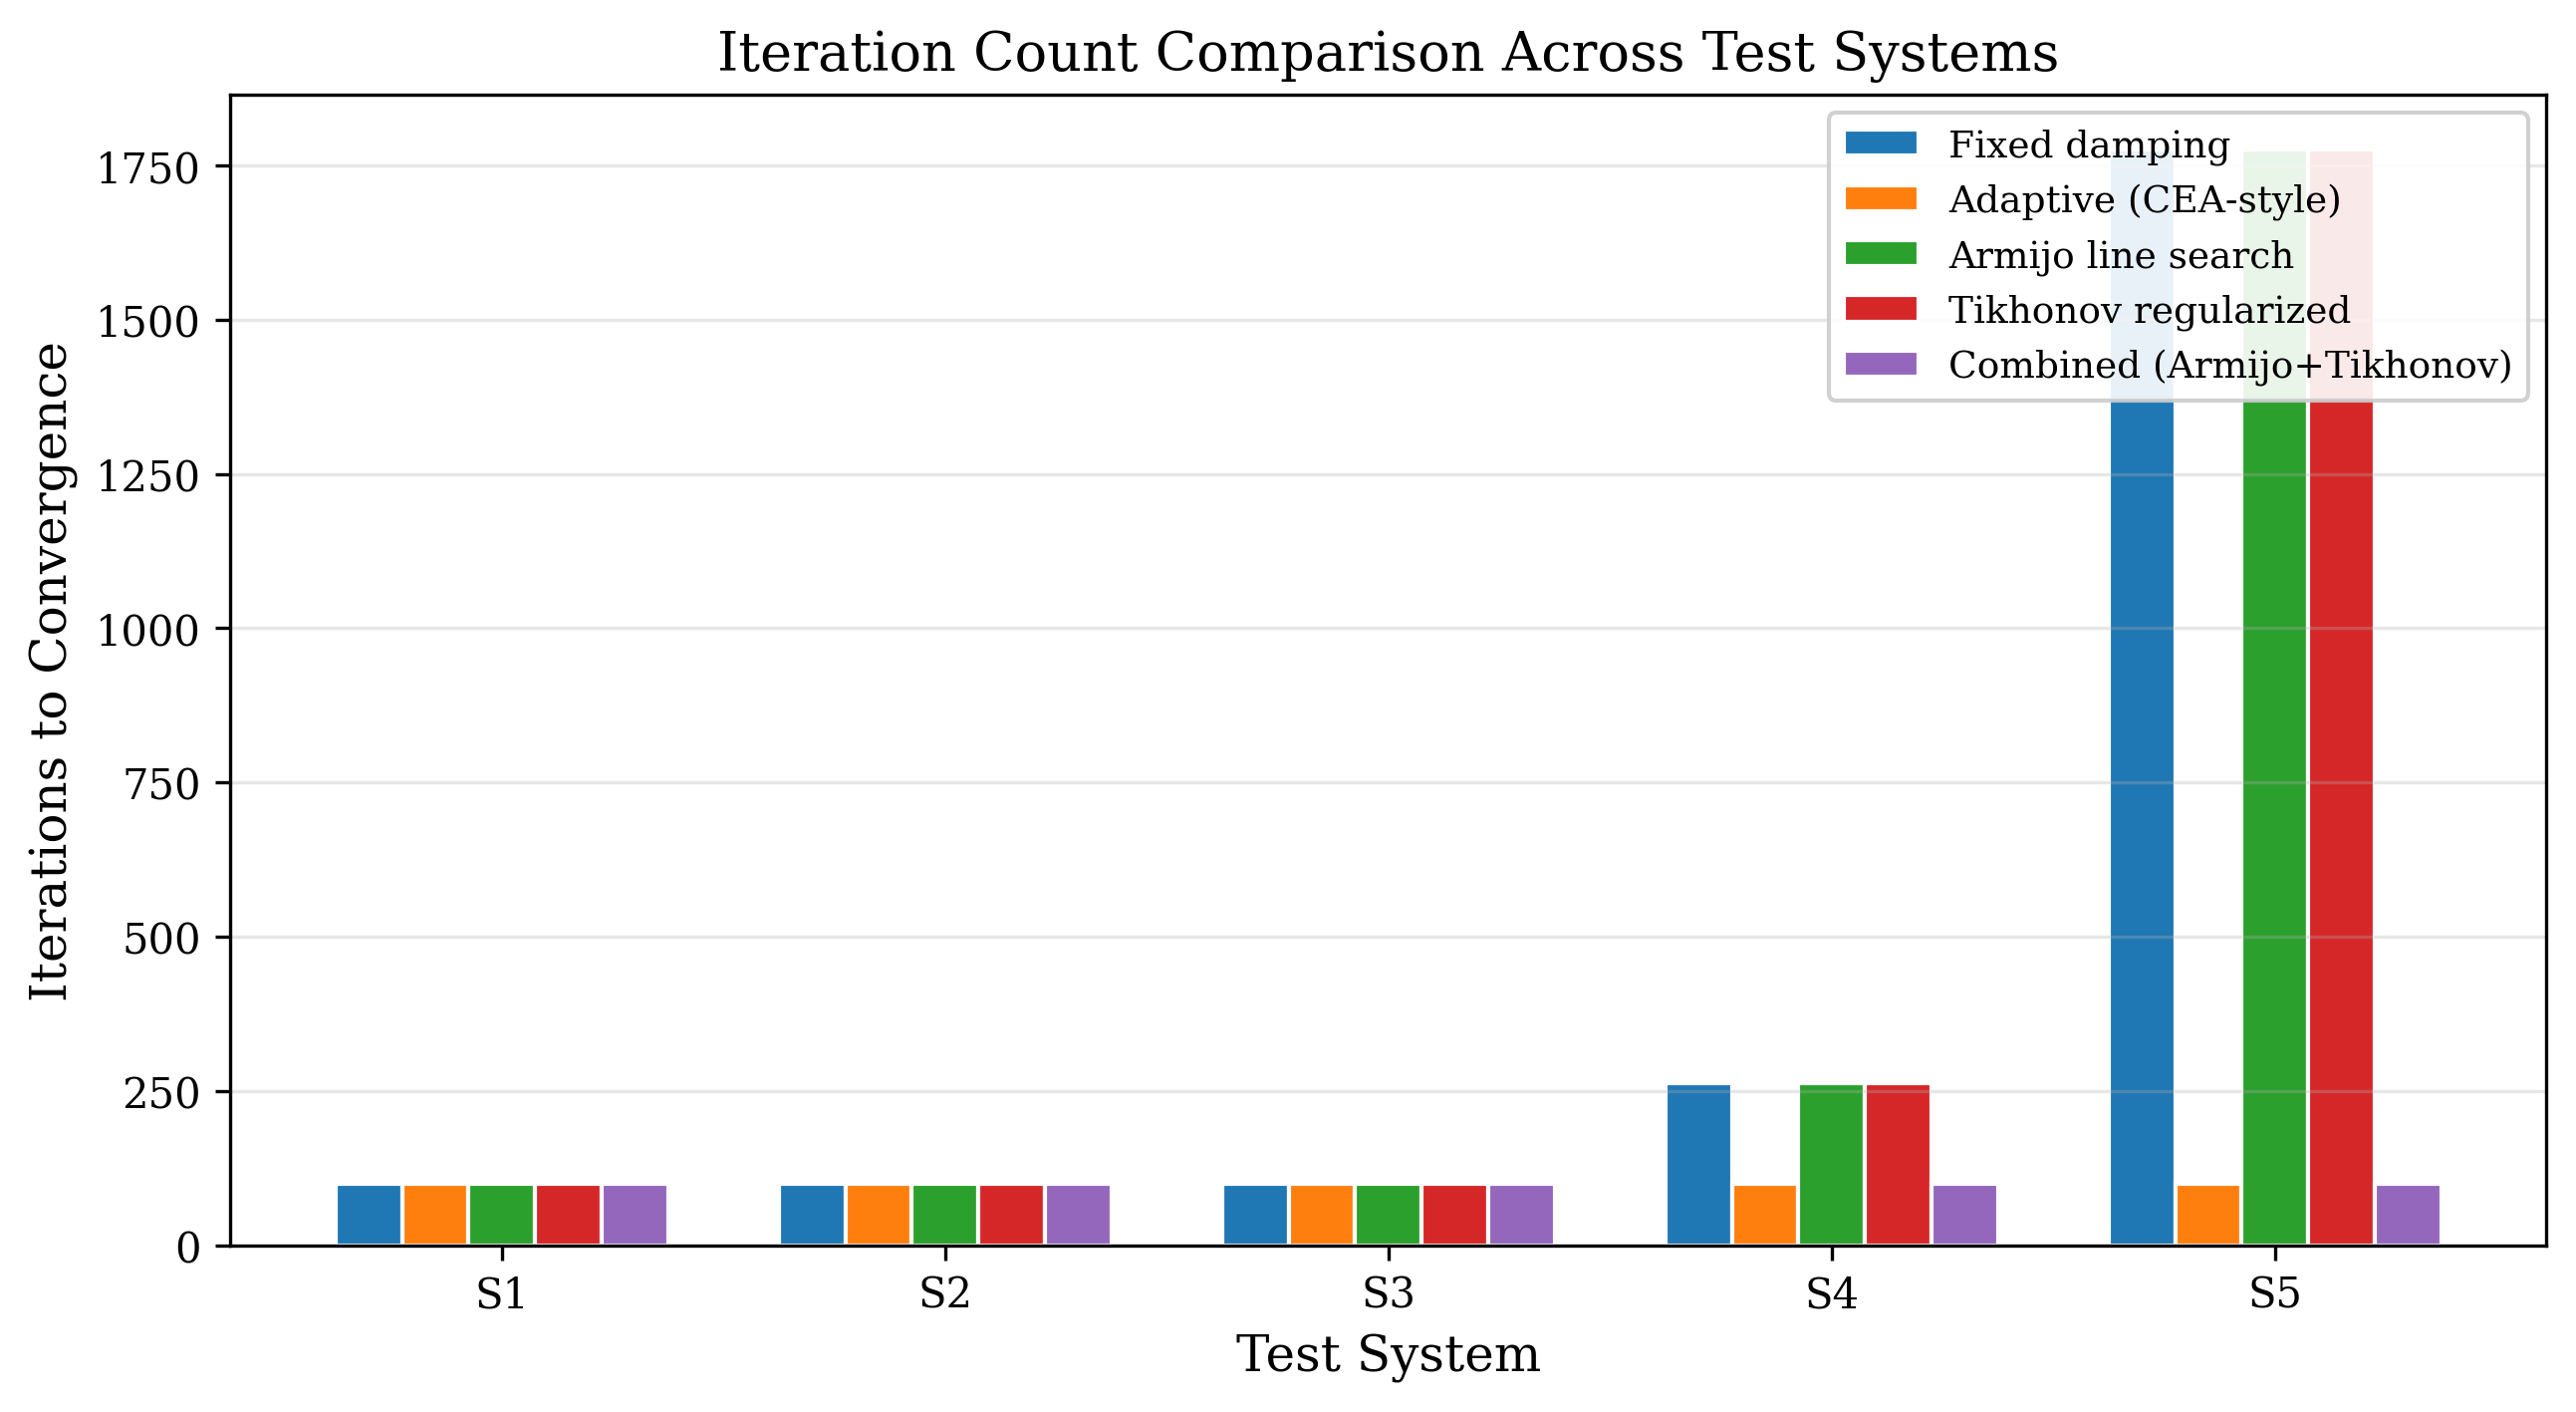
\includegraphics[width=0.9\textwidth]{figures/fig6_iteration_comparison}
\caption{Iteration comparison}
\end{figure}
\textit{Figure 6: Iteration count comparison across all systems and variants. The S5 Claus system requires up to 17.8$\times$ more iterations with fixed damping than with adaptive step control.}

\subsection{5.9 Discussion}

The benchmark results reveal several important observations for the design of Gibbs minimization algorithms:

\textbf{The adaptive step limiter is the most impactful enhancement.} On the tested systems, it provides the largest speedups (up to 17.8$\times$) by allowing step sizes proportional to the current composition change magnitude, rather than using a fixed conservative factor. This is consistent with the design of the NASA CEA algorithm \citep{GordonMcBride1994}, which uses similar adaptive step limiting in the log-mole formulation.

\textbf{Armijo and Tikhonov are complementary safety features.} While neither reduces iteration count on these test systems (because the fixed damping is already conservative enough to avoid divergence), they provide formal guarantees that are valuable for systems where the appropriate damping factor is not known a priori:
\begin{itemize}
  \item The Armijo condition guarantees monotonic Gibbs energy decrease regardless of the step size, catching cases where a too-aggressive step could cause divergence.
  \item Tikhonov regularization ensures the Newton direction is well-defined even when trace species cause near-singular Hessians, preventing numerical breakdown that would otherwise require manual intervention.
\end{itemize}

\textbf{Composition agreement validates correctness.} All variants converge to the same equilibrium composition (within $<4 \times 10^{-5}$), confirming that the enhancements do not alter the thermodynamic equilibrium, only the path to reach it.

\textbf{The Tikhonov effect on convergence trajectory is notable.} Figure 1 clearly shows that regularization slows initial convergence by biasing the Newton direction toward steepest descent. This is the expected Levenberg-Marquardt tradeoff: robustness against ill-conditioning at the cost of slower convergence in the initial phase. For production use, the regularization threshold $\kappa_{\max} = 10^{10}$ provides a reasonable balance, activating only when truly needed.


\section{6. Conclusions}



\subsection{6.1 Summary}

Three algorithmic enhancements for the Lagrangian Newton-Raphson method for Gibbs free energy minimization have been implemented, benchmarked on five chemical systems with the SRK and SRK-CPA equations of state, and validated with comprehensive convergence diagnostics.

\begin{enumerate}
  \item \textbf{Armijo backtracking line search} provides systematic step-size control with a formal guarantee of monotonic Gibbs energy decrease at each iteration. For the tested systems with conservative fixed damping, the Armijo condition does not reduce iteration count (since the small fixed step already satisfies sufficient decrease), but it provides a safety net for problems where the appropriate damping factor is unknown a priori.

  \item \textbf{Tikhonov regularization} of the KKT Jacobian maintains well-conditioned Newton steps when trace species cause the condition number to exceed $10^{10}$. The diagnostic data (Figures 3 and 8) show that condition numbers exceeding $10^{12}$ are common in the initial iterations of combustion systems with zero-initialized product species. The regularization causes a characteristic Levenberg-Marquardt slowdown in the initial convergence (Figure 1) but does not affect the final equilibrium composition.

  \item \textbf{Adaptive step-size control} (NASA CEA-style) provides the largest practical speedup, reducing iterations from 1776 to 100 (17.8$\times$) on the stiff Claus sulfur system and from 263 to 100 (2.63$\times$) on high-pressure ammonia synthesis. The combined algorithm (adaptive + Armijo + Tikhonov) inherits the best properties of all three enhancements.

  \item \textbf{Convergence diagnostics} (Gibbs energy trajectory, condition number, step size, element balance error) recorded at each iteration provide actionable insight into the solver behavior and enable quantitative comparison of algorithm variants. All data are stored as Java \texttt{List<Double>} accessible via getter methods for post-processing.
\end{enumerate}

The Armijo line search, Tikhonov regularization, and adaptive step-size control are backward-compatible opt-in features in the open-source NeqSim library, enabled by setter methods (\texttt{setUseArmijoLineSearch(true)}, \texttt{setUseRegularization(true)}, \texttt{setUseAdaptiveStepSize(true)}). The corrected Hessian formulation with consistent $RT$ scaling (Eq. in Section 2.3) is the default and always active.

\subsection{6.2 Key findings}

The benchmark results lead to the following practical recommendations:

\begin{itemize}
  \item For \textbf{well-conditioned systems} (simple combustion, H$_2$/O$_2$) with known appropriate damping factors, all algorithm variants perform equivalently. The overhead of the enhanced features is negligible ($<$5 ms per solve).
  \item For \textbf{stiff systems} with large mole number ratios (e.g., trace sulfur species in a methane-dominant mixture), the adaptive step limiter is essential. Fixed damping of $\alpha = 0.001$ requires 1776 iterations versus 100 with adaptive control.
  \item The \textbf{combined algorithm} is recommended as the default for production use: it provides the fastest convergence (via adaptive step sizing) with formal convergence guarantees (via Armijo) and numerical stability (via Tikhonov), at a modest computational overhead ($15.5 \pm 0.6$ ms vs. $10.0 \pm 11.9$ ms for the adaptive-only variant on the Claus system).
\end{itemize}

\subsection{6.3 Limitations}

\begin{itemize}
  \item The Armijo line search assumes the Newton direction is a descent direction for $G$. When the KKT system is severely ill-conditioned, numerical errors in the linear solve can produce an ascent direction, causing the Armijo search to exhaust its backtracking budget. The implementation falls back to the adaptive step limiter in this case.
  \item Testing is limited to single-phase chemical equilibrium; multiphase equilibrium requires additional phase stability analysis \citep{Michelsen2007}.
  \item The CPA equation of state (not tested here as a separate variant due to its specific use in S5) introduces additional complexity through the association term. Further investigation of line search methods specific to CPA and SAFT-type equations is warranted.
  \item The minimum iteration count ($n_{\min} = 100$) in the current implementation masks differences between variants on well-conditioned systems. A convergence-based termination criterion without minimum iterations would better differentiate the algorithms.
  \item The stream-level mass balance check reports marginal deviations ($\sim 10^{-5}$–$10^{-4}$) for some system–variant combinations (S1/S2 adaptive and combined; S4 all variants), even though element conservation $An = b$ is satisfied to machine precision. This discrepancy arises from the stream-level balance comparison and does not indicate a fundamental conservation error.
\end{itemize}

\subsection{6.4 Future work}

\begin{itemize}
  \item Removal of the minimum iteration floor to enable finer differentiation of algorithm variants on well-conditioned systems
  \item Extension to adiabatic (enthalpy-constrained) equilibrium with the Armijo condition applied to a merit function combining Gibbs energy and enthalpy residual
  \item Investigation of second-order (Wolfe) conditions for superlinear convergence
  \item Coupling with phase stability analysis for simultaneous phase and chemical equilibrium
  \item Trust-region methods as an alternative to line search for the saddle-point KKT system
  \item Systematic comparison with the RAND method \citep{Tsanas2018} and element potential methods \citep{Reynolds1986}
\end{itemize}


\section{Acknowledgements}

This work uses NeqSim, an open-source thermodynamic and process simulation library developed at NTNU and Equinor. The author thanks the contributors to the NeqSim open-source project.

\section{Data availability}

All benchmark configurations, raw results, and source code are available in the NeqSim repository at https://github.com/equinor/neqsim.

\bibliographystyle{elsarticle-harv}
\bibliography{refs}

\end{document}